\documentclass[aspectratio=169,10pt]{beamer}

% ============================================================
% Hybrid Quantum AI for Multiphysics Simulation -- seminar deck
% Madrid theme, ~33 frames. Figures live in figures/.
% Compile: latexmk -pdf hybrid_quantum_ai_seminar.tex
% ============================================================

\usetheme{Madrid}
\usecolortheme{seahorse}

\usepackage[utf8]{inputenc}
% \usepackage[T1]{fontenc}
\usepackage{amsmath,amssymb}
\usepackage{booktabs}
\usepackage{array}
\usepackage{graphicx}
\usepackage[export]{adjustbox}
\usepackage{xcolor}
\usepackage{tikz}
\usetikzlibrary{arrows.meta,positioning,calc,decorations.pathreplacing,decorations.pathmorphing}
\graphicspath{{figures/}}

\setbeamertemplate{navigation symbols}{}

\definecolor{qpurple}{HTML}{6B4C9A}
\definecolor{cblue}{HTML}{2C6E9E}
\definecolor{okgreen}{HTML}{2E7D4F}
\definecolor{warnorange}{HTML}{C9731C}
\definecolor{qred}{HTML}{B03A2E}
\definecolor{phgray}{HTML}{6E7780}

% Equation that shrinks only if wider than the text
\newcommand{\eq}[1]{\[\adjustbox{max width=0.94\linewidth}{$\displaystyle #1$}\]}

% Status tags
\newcommand{\shown}{\textcolor{okgreen}{\textbf{[Shown]}}}
\newcommand{\pending}{\textcolor{warnorange}{\textbf{[In progress]}}}
\newcommand{\planned}{\textcolor{phgray}{\textbf{[Planned]}}}

% One-line message at the bottom of a slide
\newcommand{\takeaway}[1]{%
  \vfill
  \begin{beamercolorbox}[rounded=true,shadow=false,wd=\linewidth,sep=4pt]{block title}
  \small\centering #1
  \end{beamercolorbox}}

% Figure source / caption line
\newcommand{\figcap}[1]{\par\vspace{1pt}{\scriptsize\color{phgray}#1\par}}

\title[Hybrid Quantum AI for Multiphysics]{Hybrid Quantum AI Models for Accelerating\\Multiphysics Simulation}
\subtitle{For Crystal Growth Simülations and Liquid H2 Cryogenics}
\author{Quasi AI QISKIT Seminar}
\date{October 2026}

\begin{document}

% =====================================================================
\begin{frame}
\titlepage
\end{frame}

\begin{frame}{Outline}
\tableofcontents
\end{frame}

% =====================================================================
\section{Motivation}
% =====================================================================

\begin{frame}{Multi-Physics Simulations}
\begin{columns}[T,onlytextwidth]
\column{0.56\textwidth}
\begin{itemize}\small\setlength{\itemsep}{3pt}
  \item High-fidelity coupled CFD (flow + heat + rotation + phase change) takes hours to days per run.
  \item The real cost is the \textbf{parameter sweep}: every operating point is a new simulation.
  \item Process control and digital twins need full fields in \textbf{milliseconds}.
  \item Classical surrogates (PINN, PINO) help, but stall on sharp, strongly coupled fields.
\end{itemize}
\vspace{0.15cm}
\begin{block}{Goal}
\small A surrogate that keeps the governing physics, generalises across operating conditions, and evaluates in real time.
\end{block}
\column{0.40\textwidth}
\centering
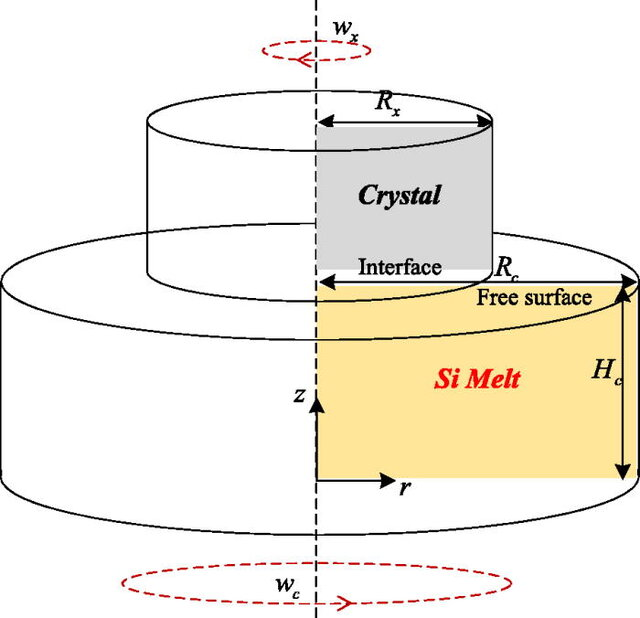
\includegraphics[width=\linewidth,height=0.62\textheight,keepaspectratio]{Simulation-region-of-silicon-single-crystal-growth_W640.jpg}
\figcap{Czochralski (CZ) growth: rotating crystal ($\omega_s$) pulled from a Si melt in a counter-rotating crucible ($\omega_c$).}
\end{columns}
\end{frame}

\begin{frame}{Two industrial use cases}
\begin{columns}[T,onlytextwidth]
\column{0.58\textwidth}
\begin{block}{Silicon crystal growth (Czochralski)}
\footnotesize Melt convection, swirl and the thermal field (1685--1750\,K) set defect density and oxygen uptake. \textbf{Aim:} fast field prediction to tune the process.
\end{block}
\vspace{0.05cm}
\centering
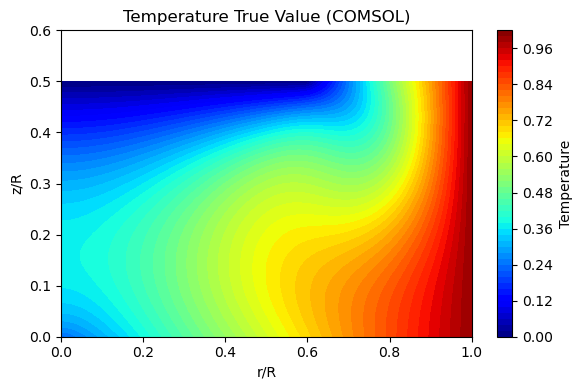
\includegraphics[width=0.49\linewidth]{temp.png}\hfill
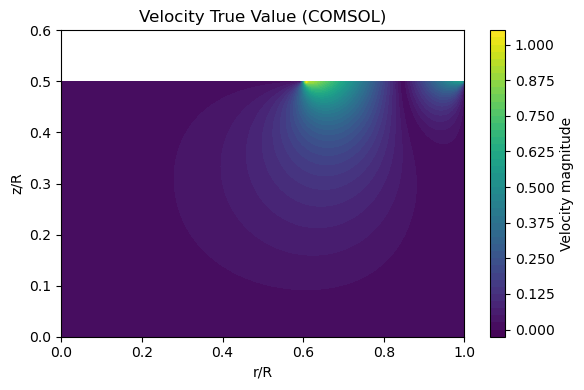
\includegraphics[width=0.49\linewidth]{velocity.png}
\figcap{COMSOL reference: temperature (left) and velocity magnitude (right) in the melt. Sharp gradients sit at the free surface and crystal edge.}
\column{0.38\textwidth}
\begin{block}{LH$_2$ cryogenic boil-off}
\begin{itemize}\footnotesize
  \item Heat leak into liquid-hydrogen tanks ($\approx$20\,K) drives natural convection, stratification and evaporation.
  \item Turbulent convection with phase change and a \textbf{moving liquid--vapour interface}.
  \item \textbf{Aim:} predict boil-off rate and pressure rise for tank design.
\end{itemize}
\end{block}
\begin{exampleblock}{Common thread}
\footnotesize Strongly coupled, non-linear transport of velocity, temperature, species and interfaces.
\end{exampleblock}
\end{columns}
\end{frame}

\begin{frame}{Our proposal in one slide}
\begin{enumerate}\setlength{\itemsep}{4pt}
  \item \textbf{Problem:} classical PINNs suffer from spectral bias, loss imbalance and badly scaled coupled fields.
  \item \textbf{Framework:} Hybrid-QPINN / QPINO, a classical network with a shallow parameterised quantum circuit (PQC) as a trainable feature map, fed by Fourier features and data re-uploading.
  \item \textbf{Target physics:} strongly coupled non-linear transport: velocity, temperature, and next concentration and evolving interfaces.
  \item \textbf{Benchmarks:} silicon CZ crystal growth (running) and LH$_2$ boil-off (defined).
  \item \textbf{Destination:} real-time digital twins and fast parametric exploration.
\end{enumerate}
%\vspace{0.2cm}
%\begin{alertblock}{How to read the results}
%Each claim carries a status: \shown{} measured, \pending{} experiment running, \planned{} designed but not yet run.
%\end{alertblock}
\end{frame}

% =====================================================================
\section{classical PINNs}
% =====================================================================

\begin{frame}{Physics-informed neural networks}
\begin{columns}[T,onlytextwidth]
\column{0.52\textwidth}
\begin{itemize}\small
  \item A network $\hat u_\theta(x)$ is trained so that the PDEs and boundary/initial conditions hold.
  \item Derivatives come from automatic differentiation: no mesh, no stencil.
\end{itemize}
\eq{\mathcal{L} = \mathcal{L}_{\mathrm{data}} + \lambda_{\mathrm{PDE}}\mathcal{L}_{\mathrm{PDE}} + \lambda_{\mathrm{BC}}\mathcal{L}_{\mathrm{BC}} + \lambda_{\mathrm{IC}}\mathcal{L}_{\mathrm{IC}}}
\begin{itemize}\small
  \item Strength: little labelled data, natural fit for coupled equations.
  \item Limitation: one PINN = one operating point. Neural operators (PINO) learn whole solution families.
\end{itemize}
\column{0.44\textwidth}
\centering
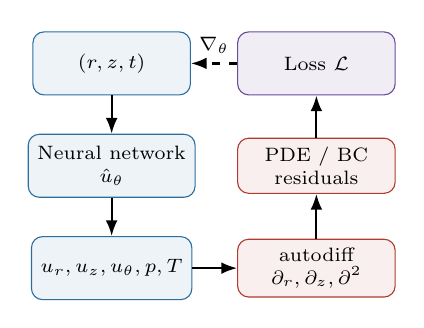
\begin{tikzpicture}[font=\scriptsize,
  b/.style={rounded corners,draw=cblue,fill=cblue!8,minimum width=2.0cm,minimum height=0.8cm,align=center},
  r/.style={rounded corners,draw=qred,fill=qred!8,minimum width=2.0cm,minimum height=0.7cm,align=center},
  arr/.style={-{Latex[length=2mm]},thick}]
\node[b] (x) at (0,0) {$(r,z,t)$};
\node[b] (n) at (0,-1.3) {Neural network\\$\hat u_\theta$};
\node[b] (u) at (0,-2.6) {$u_r,u_z,u_\theta,p,T$};
\node[r] (ad) at (2.6,-2.6) {autodiff\\$\partial_r,\partial_z,\partial^2$};
\node[r] (res) at (2.6,-1.3) {PDE / BC\\residuals};
\node[b,draw=qpurple,fill=qpurple!10] (L) at (2.6,0) {Loss $\mathcal{L}$};
\draw[arr] (x)--(n); \draw[arr] (n)--(u); \draw[arr] (u)--(ad);
\draw[arr] (ad)--(res); \draw[arr] (res)--(L);
\draw[arr,dashed] (L.west)--node[above]{$\nabla_\theta$}(x.east);
\end{tikzpicture}
\end{columns}
\end{frame}

\begin{frame}{Bottleneck 1: spectral bias}
\begin{columns}[T,onlytextwidth]
\column{0.42\textwidth}
\begin{itemize}\small\setlength{\itemsep}{3pt}
  \item MLPs learn low frequencies first; sharp content converges slowly (Rahaman et al., 2019).
  \item Transport fields are full of sharp structure: thermal boundary layers, wall shear, swirl near rotating walls, phase interfaces.
  \item Classical remedy: Fourier feature inputs (Tancik et al., 2020).
  \item \textbf{Our addition:} a \emph{trainable} quantum feature map whose outputs are trigonometric polynomials of its inputs.
\end{itemize}
\column{0.56\textwidth}
\centering
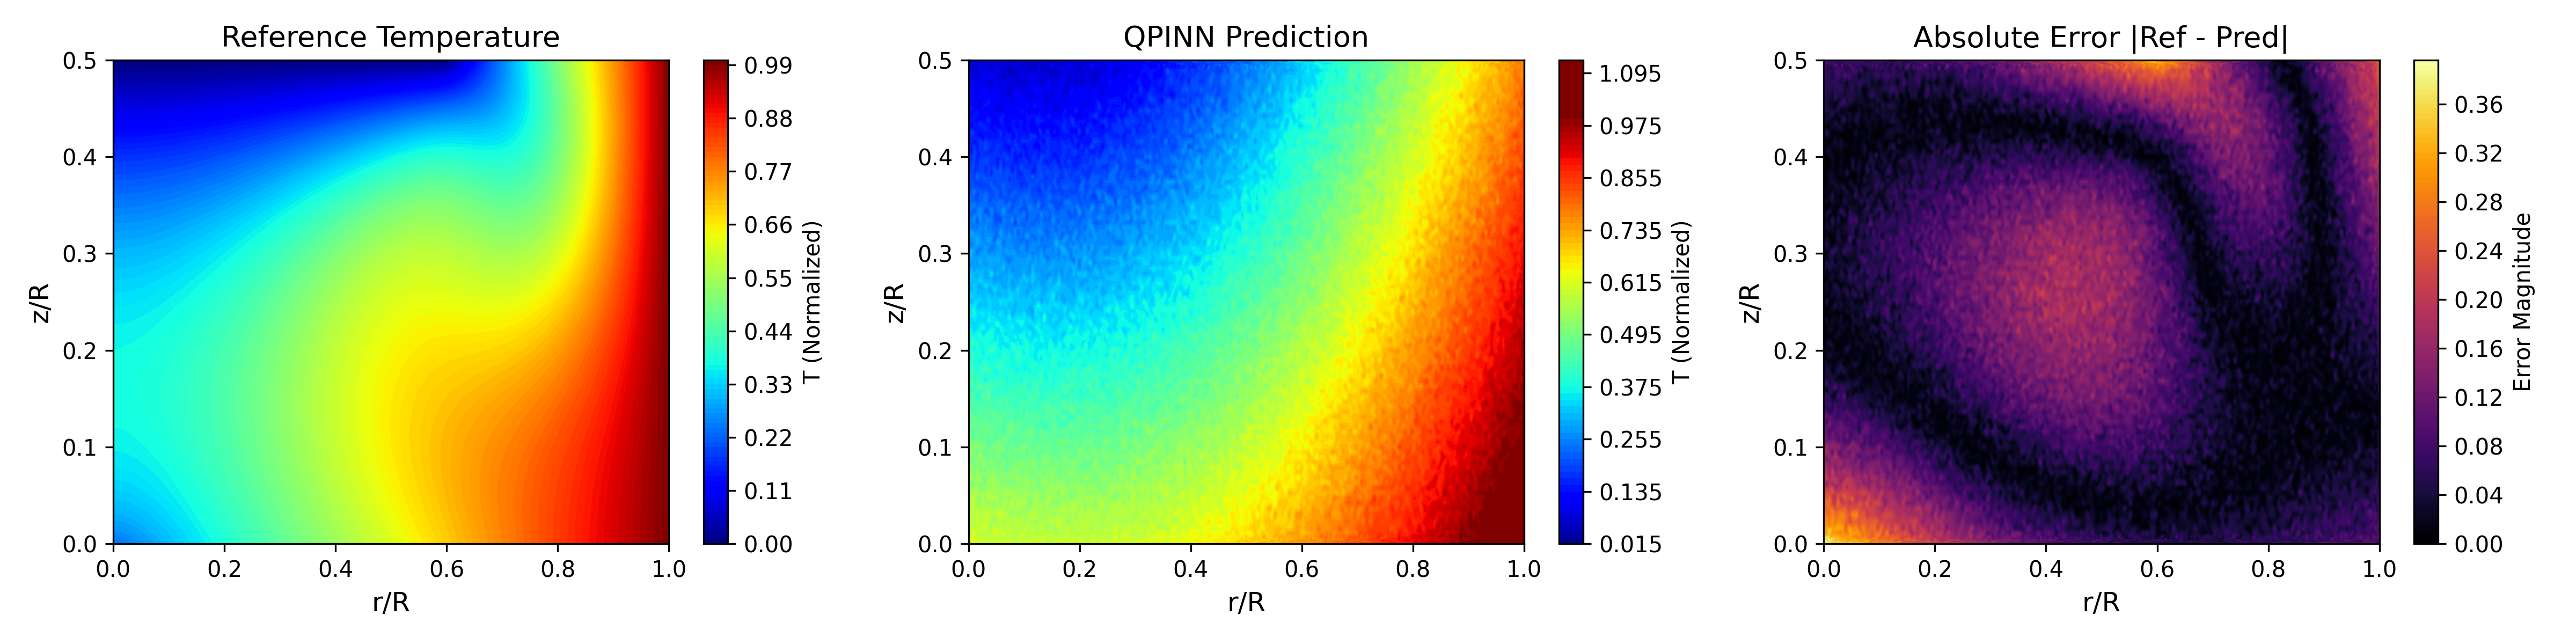
\includegraphics[width=\linewidth]{qpinn_comparison_error.png}
\figcap{Reference temperature, a smooth network prediction, and the absolute error. The error concentrates on the curved thermal front, exactly where the field carries high-frequency content.}
\end{columns}
\end{frame}

%============================================================
\section{Improved PINNs for Silicon Crystal Growth}
%============================================================
\begin{frame}{Use case: Czochralski (CZ) silicon crystal growth}
\begin{columns}[T,onlytextwidth]
\column{0.29\textwidth}
\centering
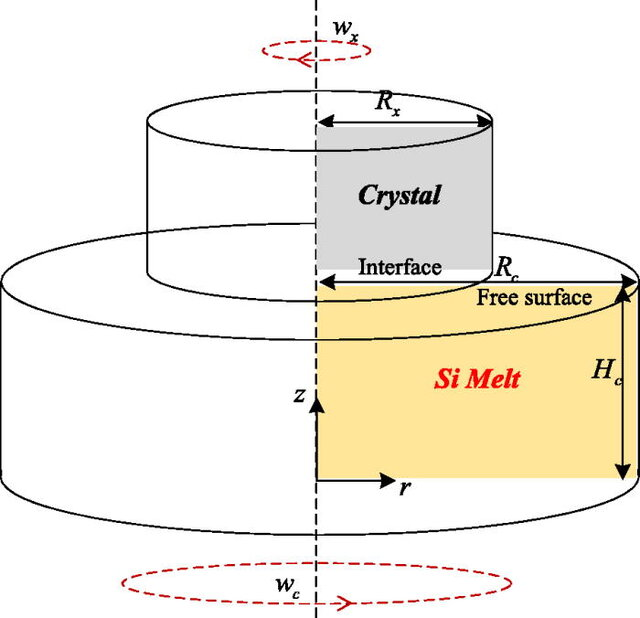
\includegraphics[width=\linewidth]{Simulation-region-of-silicon-single-crystal-growth_W640.jpg}\\[-0.5mm]
\figsrc{Axisymmetric melt domain in $(r,z)$}
\column{0.40\textwidth}
\begin{itemize}\small
  \item A seed crystal is pulled from molten silicon; crystal ($\omega_s$) and crucible ($\omega_c$) rotate.
  \item Coupled physics: Navier--Stokes + energy, Boussinesq buoyancy, rotating walls ($u_\theta=\omega r$).
  \item Five unknown fields per point: $u_r,\,u_z,\,u_\theta,\,p,\,T$.
  \item These thermal and flow fields largely determine crystal quality.
\end{itemize}
\column{0.27\textwidth}
\centering
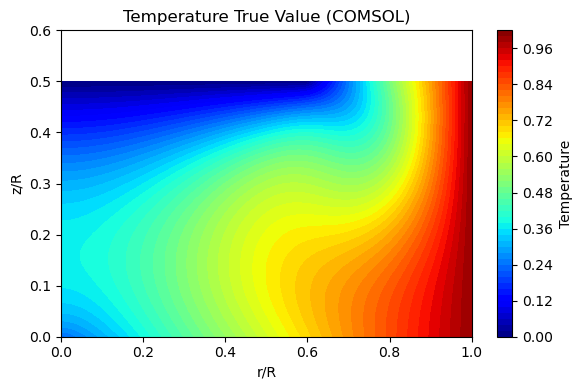
\includegraphics[height=2.35cm]{temp.png}\\
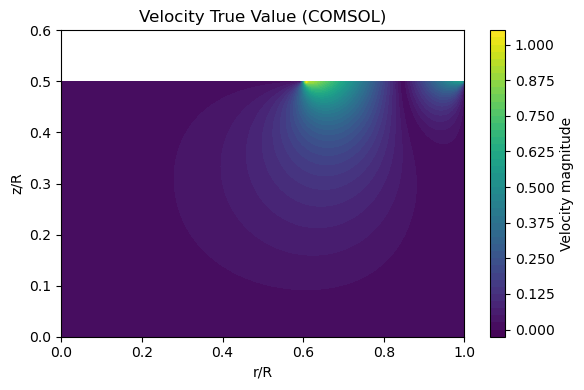
\includegraphics[height=2.35cm]{velocity.png}\\[-0.5mm]
\figsrc{Reference $T$ and $|\mathbf u|$ (normalised, COMSOL)}
\end{columns}
\takeaway{Accurate CFD exists, but sweeping process settings (rotation, heater temperature) with it is slow.}
\end{frame}

\begin{frame}{Physics-informed neural networks (PINNs) in one slide}
\begin{columns}[T,onlytextwidth]
\column{0.50\textwidth}
\centering
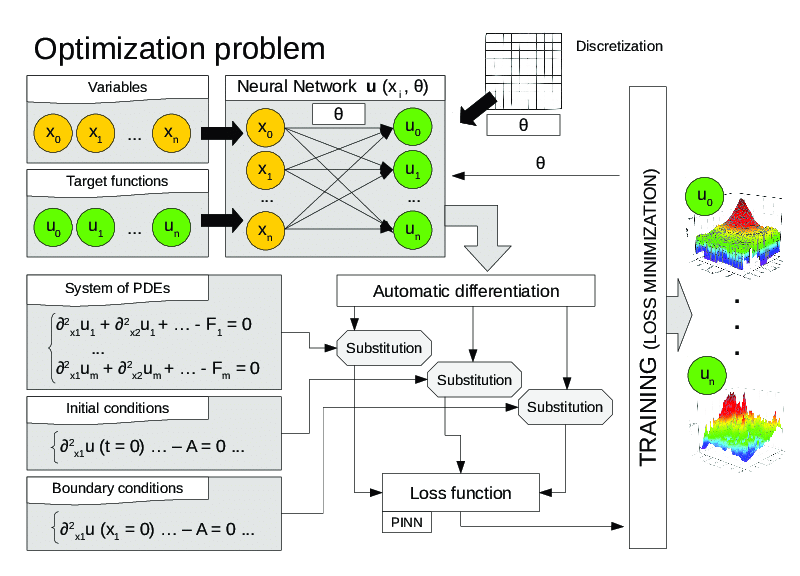
\includegraphics[width=\linewidth,height=5.0cm,keepaspectratio,trim=0 0 42 0,clip]{pinns_2.png}\\[-0.5mm]
\figsrc{Network $\rightarrow$ automatic differentiation $\rightarrow$ PDE/BC/IC residuals $\rightarrow$ loss}
\column{0.47\textwidth}
\begin{enumerate}\small
  \item A neural network $\hat u_\theta(x,t)$ represents the solution.
  \item Automatic differentiation gives exact derivatives, so the PDE residual can be evaluated at any point.
  \item One loss combines PDE, boundary (BC) and initial (IC) terms:
\end{enumerate}
\vspace{-1mm}
\[
\mathcal L=\lambda_{\mathrm{PDE}}\,\mathcal L_{\mathrm{PDE}}+\lambda_{\mathrm{BC/IC}}\,\mathcal L_{\mathrm{BC/IC}}
\]
\vspace{-3mm}
\begin{alertblock}{The catch}
\small The terms have very different gradient scales, so the weights $\lambda$ decide what the network actually learns.
\end{alertblock}
\end{columns}
\takeaway{Physics enters through the loss, so less labelled data is needed; but the loss balance must be handled with care.}
\end{frame}

\begin{frame}{Study design: two questions about trust}
\begin{columns}[T,onlytextwidth]
\column{0.48\textwidth}
\begin{block}{A.\ Adaptive PINN training}
\small \textbf{Question:} if the loss weights adapt during training, is a lower PDE loss a better solution?
\begin{itemize}\small
  \item \key{Baseline PINN}: fixed unit weights.
  \item \key{GNPINN}: normalises the PDE and BC/IC gradients.
  \item \key{AgenticPINN}: a rule-based controller re-weights the loss terms.
\end{itemize}
\small Tested on the 1D heat equation (exact solution known) and a simplified CZ thermal-fluid PINN.
\end{block}
\column{0.48\textwidth}
\begin{block}{B.\ CFD surrogate (Gaussian process)}
\small \textbf{Question:} how well does a surrogate predict a \emph{whole unseen} operating condition, field by field?
\begin{itemize}\small
  \item 33 ANSYS Fluent reference cases: steady, laminar, 2D axisymmetric, 8181 nodes.
  \item Three one-parameter sweeps: heater-wall temperature $T_{\mathrm{hot}}$, crucible rotation $\omega_c$, crystal rotation $\omega_s$.
  \item One complete case per sweep is held out for testing.
\end{itemize}
\end{block}
\end{columns}
\takeaway{Fair tests: in A only the training strategy changes; in B the test is a new process setting, not random points of known cases.}
\end{frame}

\begin{frame}{Classical PINN baseline on simplified crystal growth}
\begin{columns}[T,onlytextwidth]
\column{0.38\textwidth}
\centering
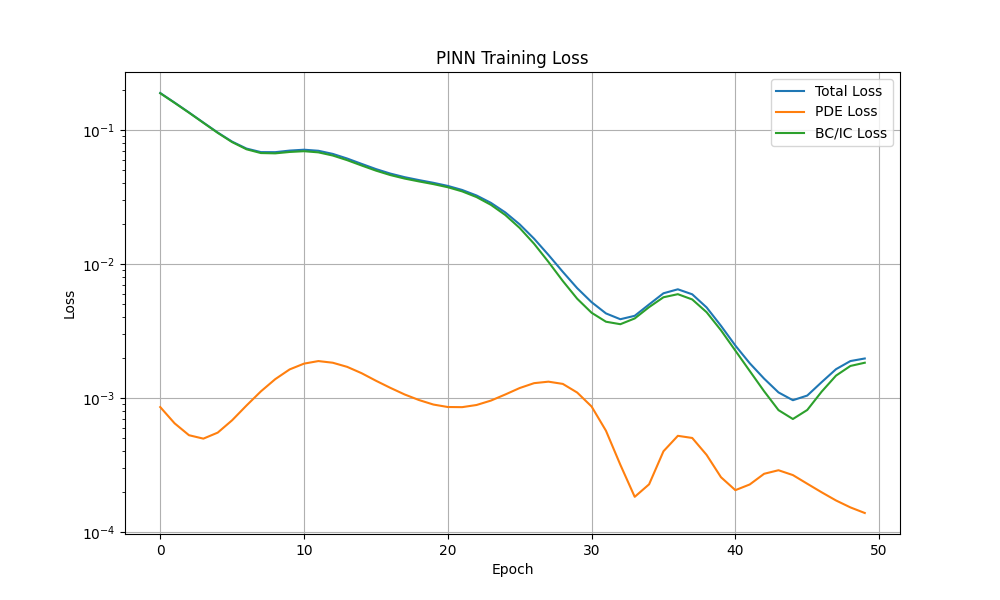
\includegraphics[width=\linewidth]{crystal_growth_loss.png}
\figcap{Training loss: total, PDE and BC/IC components (50 epochs).}
\vspace{0.1cm}
\begin{itemize}\footnotesize
  \item Total loss is driven by BC/IC; the PDE term oscillates rather than falling steadily.
  \item Loss ends rising again after epoch 45.
\end{itemize}
\column{0.60\textwidth}
\centering
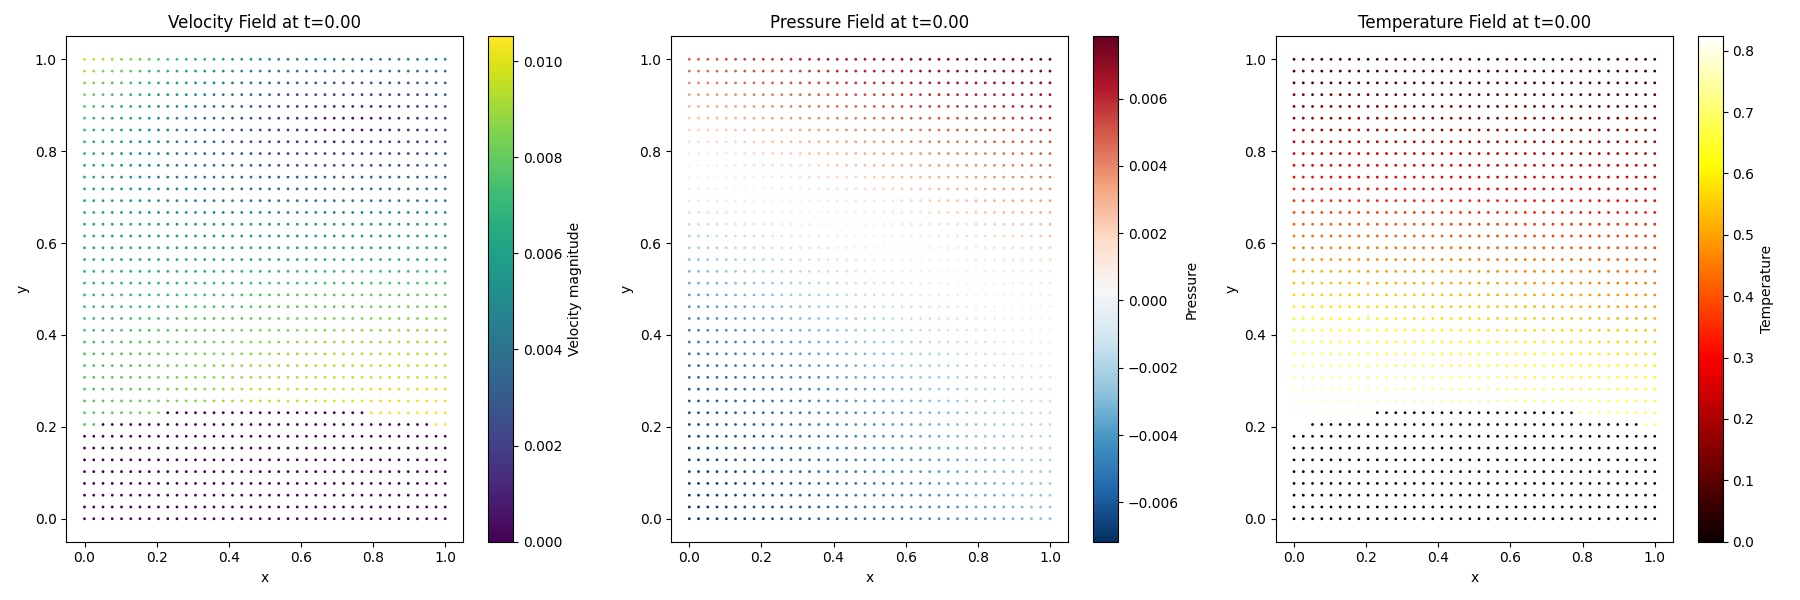
\includegraphics[width=\linewidth]{crystal_growth_t0_0.png}\\[-1pt]
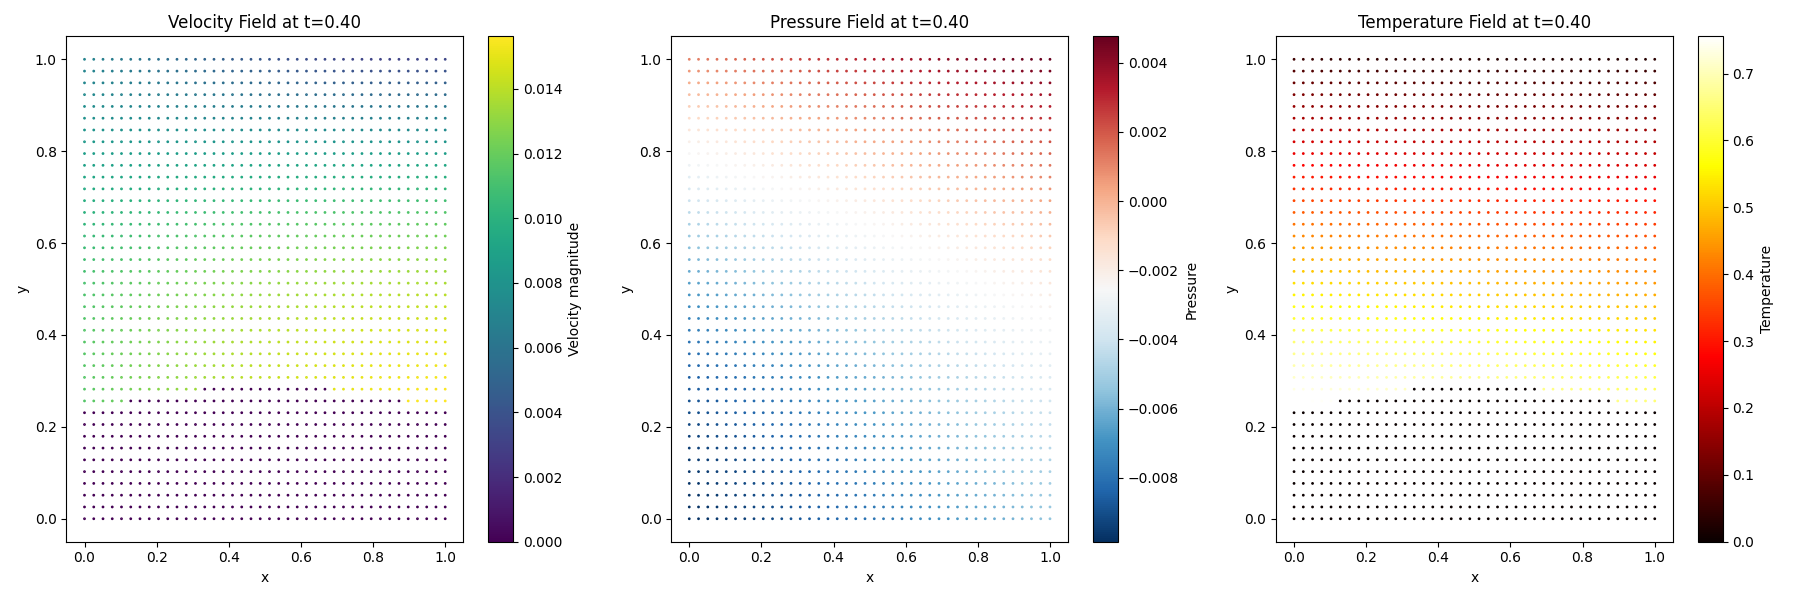
\includegraphics[width=\linewidth]{crystal_growth_t0_4.png}
\figcap{Predicted velocity, pressure and temperature at $t=0$ (top) and $t=0.4$ (bottom). Fields stay diffuse; the near-interface layer is barely resolved.}
\end{columns}
\end{frame}

\begin{frame}{Bottleneck 2: loss-term imbalance}
\begin{columns}[T,onlytextwidth]
\column{0.50\textwidth}
\begin{center}
\footnotesize
\begin{tabular}{lccc}
\toprule
Trainer (1D heat) & PDE loss & BC/IC loss & Rel.\ $L_2$ \\
\midrule
Baseline    & $3.96\!\times\!10^{-3}$ & $1.15\!\times\!10^{-3}$ & $0.084$ \\
GNPINN      & $9.74\!\times\!10^{-3}$ & $\mathbf{9.05\!\times\!10^{-4}}$ & $\mathbf{0.054}$ \\
AgenticPINN & $\mathbf{8.22\!\times\!10^{-7}}$ & $2.00\!\times\!10^{-1}$ & \textcolor{qred}{$\mathbf{1.368}$} \\
\bottomrule
\end{tabular}
\end{center}
\begin{itemize}\footnotesize
  \item The term with the largest raw gradient dominates (Wang et al., 2021).
  \item AgenticPINN: PDE residual $\approx$4800$\times$ smaller, BC/IC $\approx$173$\times$ larger, and the field is wrong.
\end{itemize}
\begin{block}{Lesson carried into this work}
\footnotesize Report loss components and per-field errors, never only a weighted total.
\end{block}
\column{0.47\textwidth}
\centering
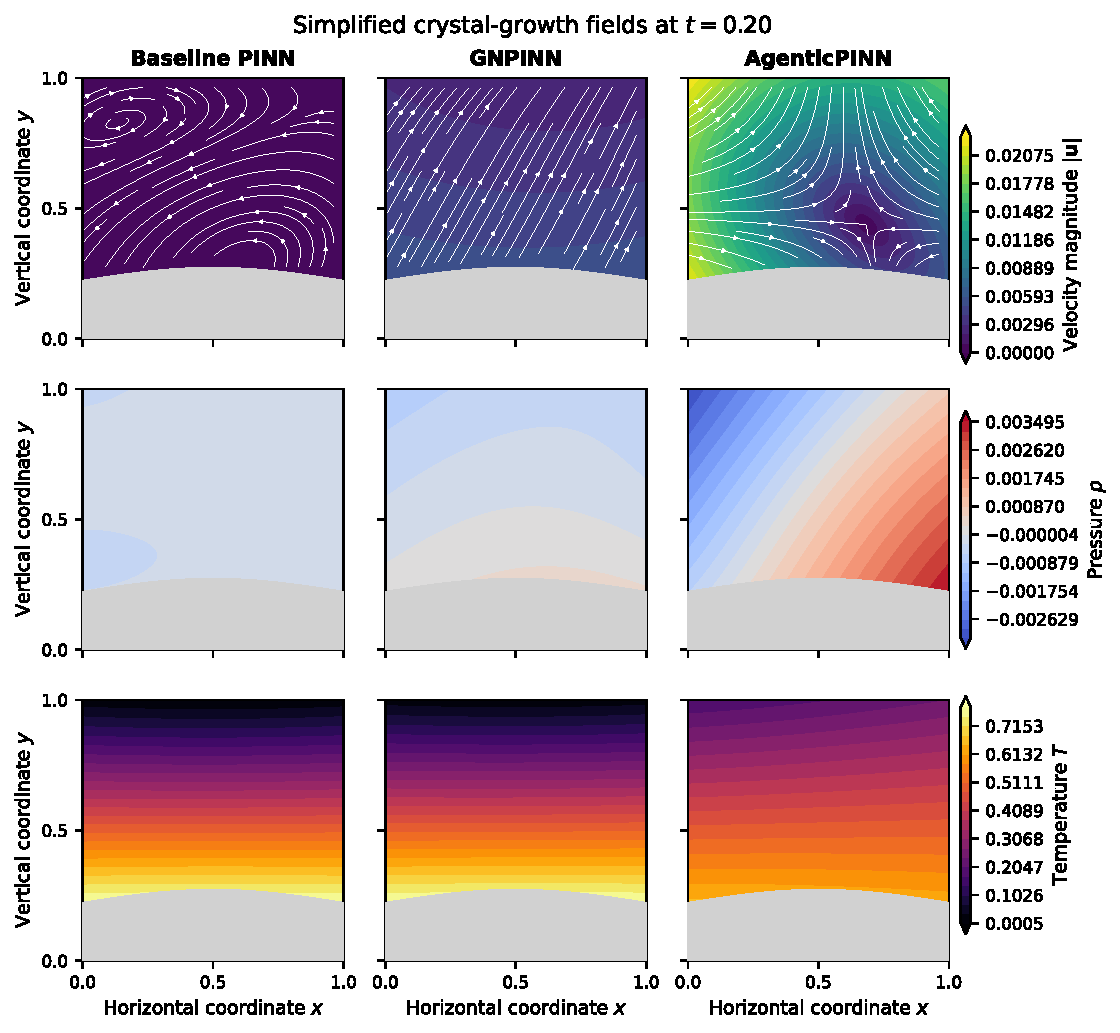
\includegraphics[width=\linewidth,height=0.72\textheight,keepaspectratio]{crystal_mlp_fields.pdf}
\figcap{Simplified CZ fields at $t=0.2$: baseline PINN, GNPINN, AgenticPINN (velocity, pressure, temperature). Chapagain et al., 2026.}
\end{columns}
\end{frame}

\begin{frame}{Bottleneck 3: scale mismatch between coupled fields}
\begin{columns}[T,onlytextwidth]
\column{0.55\textwidth}
\begin{itemize}
  \item Five coupled outputs: $u_r, u_z, u_\theta, p, T$, with very different magnitudes.
  \item In the CZ model the pressure coefficient is
  \[p_{\mathrm{coeff}} = \frac{p_{\mathrm{scale}}}{v_{\mathrm{scale}}^2} = 134{,}128.\]
  \item Viscous terms scale as $1/Re \approx 0.067$.
  \item Pressure-to-viscous ratio $\approx 2\times10^{6}:1$.
\end{itemize}
\column{0.41\textwidth}
\begin{alertblock}{Consequence}
The pressure residual can overwhelm the data signal during physics-informed training. This is the main stability issue we measured (Result 3).
\end{alertblock}
\vspace{0.2cm}
\begin{block}{Design response}
Hard constraints, staged physics warm-up, EMA residual balancing, and next per-field residual scaling.
\end{block}
\end{columns}
\end{frame}

% =====================================================================
\section{The Hybrid Quantum AI Models}
% =====================================================================

\begin{frame}{Architecture overview}
\centering
\resizebox{\linewidth}{!}{%
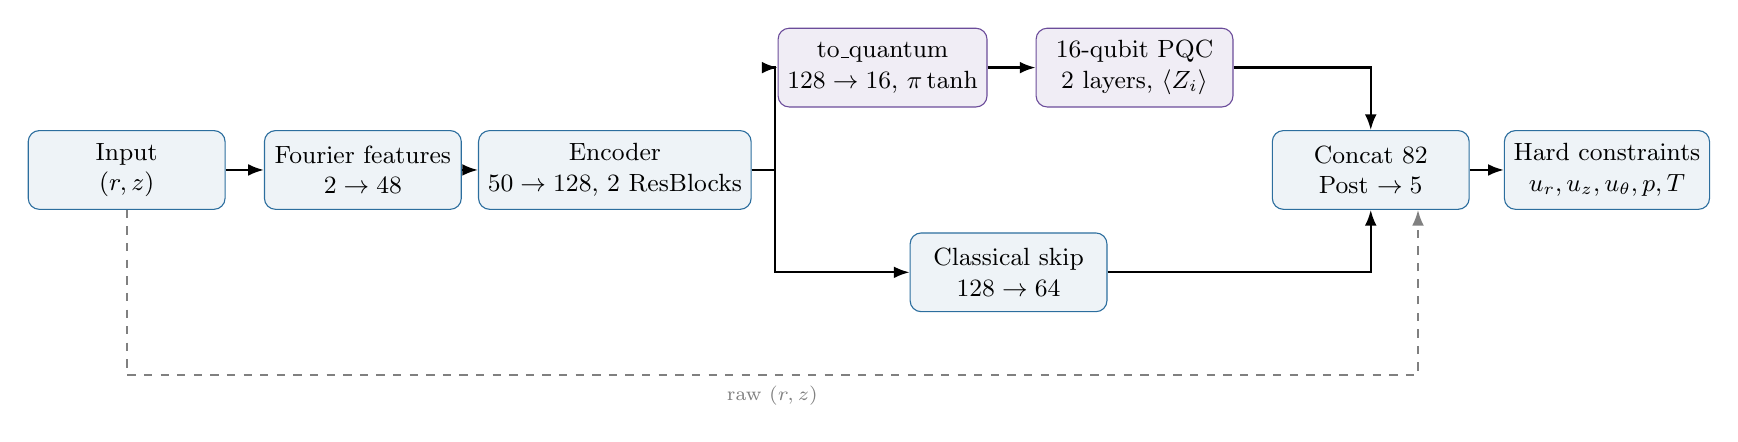
\begin{tikzpicture}[
  font=\small,
  cls/.style={rounded corners,draw=cblue,fill=cblue!8,minimum height=1.0cm,minimum width=2.5cm,align=center},
  qnt/.style={rounded corners,draw=qpurple,fill=qpurple!10,minimum height=1.0cm,minimum width=2.5cm,align=center},
  arr/.style={-{Latex[length=2mm]},thick}
]
\node[cls] (in) at (0,0) {Input\\$(r,z)$};
\node[cls] (ff) at (3.0,0) {Fourier features\\$2\to48$};
\node[cls] (enc) at (6.2,0) {Encoder\\$50\to128$, 2 ResBlocks};
\node[qnt] (tq) at (9.6,1.3) {to\_quantum\\$128\to16$, $\pi\tanh$};
\node[qnt] (pqc) at (12.8,1.3) {16-qubit PQC\\2 layers, $\langle Z_i\rangle$};
\node[cls] (sk) at (11.2,-1.3) {Classical skip\\$128\to64$};
\node[cls] (post) at (15.8,0) {Concat 82\\Post $\to5$};
\node[cls] (out) at (18.8,0) {Hard constraints\\$u_r,u_z,u_\theta,p,T$};
\draw[arr] (in)--(ff); \draw[arr] (ff)--(enc);
\draw[arr] (enc.east)--++(0.3,0)|-(tq.west);
\draw[arr] (enc.east)--++(0.3,0)|-(sk.west);
\draw[arr] (tq)--(pqc);
\draw[arr] (pqc.east)-|(post.north);
\draw[arr] (sk.east)-|(post.south);
\draw[arr] (post)--(out);
\draw[arr,dashed,gray] (in.south)--++(0,-2.1)-|node[pos=0.25,below,font=\scriptsize]{raw $(r,z)$} ([xshift=0.6cm]post.south);
\end{tikzpicture}}

\vspace{0.3cm}
\begin{columns}[T,onlytextwidth]
\column{0.32\textwidth}
\begin{block}{Classical backbone}
\footnotesize Fourier encoding plus residual MLP: carries most of the computation.
\end{block}
\column{0.32\textwidth}
\begin{exampleblock}{Quantum feature map}
\footnotesize 16 qubits, 2 layers, 96 trainable angles; 16 expectation values out.
\end{exampleblock}
\column{0.32\textwidth}
\begin{block}{Skip path}
\footnotesize The head never depends solely on the quantum bottleneck.
\end{block}
\end{columns}
\end{frame}

\begin{frame}{Ingredient 1: Fourier feature mapping}
\begin{columns}[T,onlytextwidth]
\column{0.54\textwidth}
\begin{itemize}\small
  \item Frozen random matrix $B\in\mathbb{R}^{2\times24}$, $B_{ij}\sim\mathcal{N}(0,6^2)$.
  \eq{\gamma(x) = \big[\sin(2\pi\,xB),\ \cos(2\pi\,xB)\big]\in\mathbb{R}^{48}}
  \item Frequencies span roughly $\pm15$ cycles per unit length in normalised coordinates.
  \item Concatenated with raw $(r,z)$: 50 inputs to the encoder.
  \item High-frequency access from the first layer, at \textbf{zero trainable cost}.
\end{itemize}
\column{0.42\textwidth}
\centering
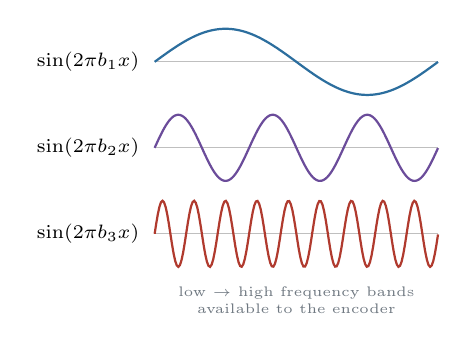
\begin{tikzpicture}[x=3.6cm,y=0.42cm,font=\scriptsize]
\foreach \f/\yo/\c [count=\i] in {1/0/cblue,3/-2.6/qpurple,9/-5.2/qred}{
  \draw[gray!50] (0,\yo)--(1,\yo);
  \draw[thick,\c,domain=0:1,samples=180] plot (\x,{\yo+sin(\f*360*\x)});
  \node[anchor=east] at (-0.02,\yo) {$\sin(2\pi b_{\i}x)$};
}
\node[font=\tiny,text=phgray,align=center] at (0.5,-7.2) {low $\rightarrow$ high frequency bands\\available to the encoder};
\end{tikzpicture}
\end{columns}
\end{frame}

\begin{frame}{Ingredient 2: shallow parameterised quantum circuit}
\begin{columns}[T,onlytextwidth]
\column{0.50\textwidth}
\centering
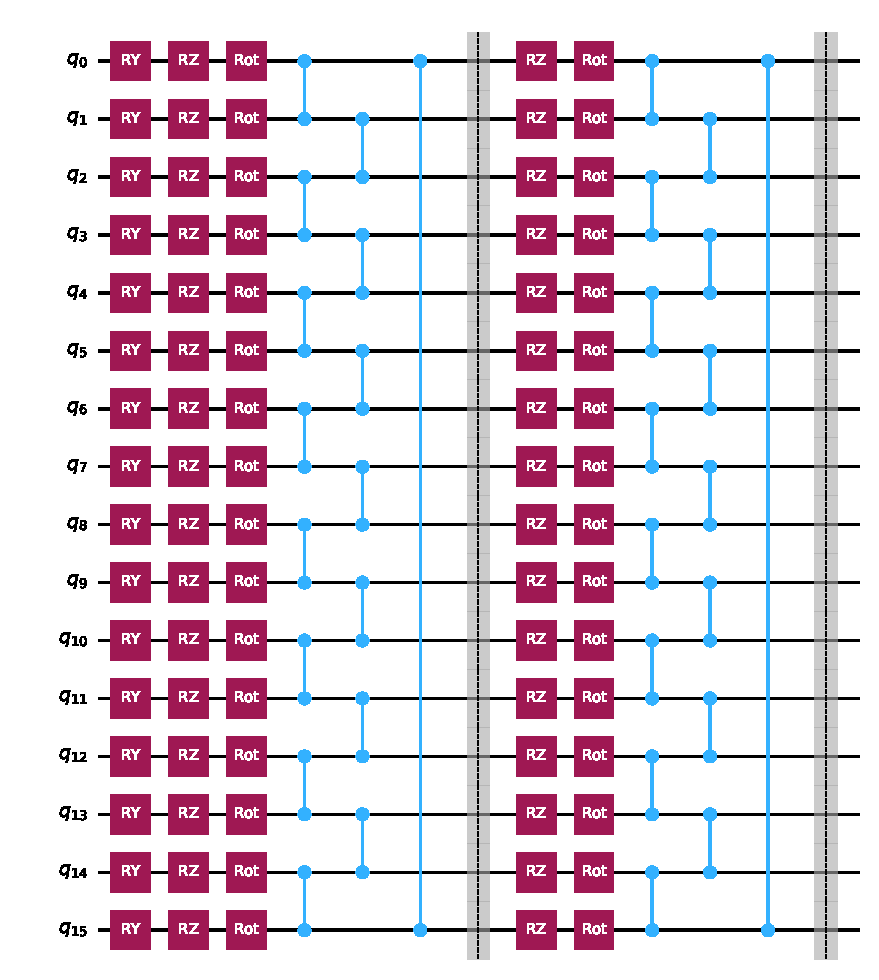
\includegraphics[width=\linewidth,height=0.80\textheight,keepaspectratio]{circuit_logical.pdf}
\figcap{Logical circuit, 16 qubits $\times$ 2 layers.}
\column{0.47\textwidth}
\begin{enumerate}\small\setlength{\itemsep}{2pt}
  \item \textbf{Encode:} $R_Y(\theta_i)$, $\theta_i=\pi\tanh(h_i)\in[-\pi,\pi]$.
  \item \textbf{Re-upload:} $R_Z(0.5\,\theta_{(i+\ell)\bmod16})$.
  \item \textbf{Train:} $\mathrm{Rot}(\varphi_i,\vartheta_i,\omega_i)$, 48 angles per layer.
  \item \textbf{Entangle:} CZ ring, closing $q_{15}$--$q_0$.
\end{enumerate}
\vspace{0.15cm}
\begin{block}{Readout}
\small $\langle Z_i\rangle$, $i=0,\dots,15$ $\to$ LayerNorm(16).\\
\textbf{96 trainable quantum parameters}, about 50 gates per shot on hardware.
\end{block}
\end{columns}
\end{frame}

\begin{frame}{Ingredient 3: data re-uploading}
\begin{columns}[T,onlytextwidth]
\column{0.55\textwidth}
\begin{itemize}\small\setlength{\itemsep}{3pt}
  \item A PQC output is a truncated Fourier series of its encoded input (Schuld et al., 2021):
  \eq{f_\phi(\theta) = \sum_{\omega\in\Omega_L} c_\omega(\phi)\, e^{i\omega\theta}}
  \item Encoding once gives a narrow spectrum $\Omega_1$; re-uploading in every layer widens it to $\Omega_L$ (P\'erez-Salinas et al., 2020).
  \item The cyclic shift $\theta_{(i+\ell)\bmod16}$ lets each layer mix a different combination of latent features.
  \item With Fourier inputs, this targets exactly the content that spectral bias suppresses.
\end{itemize}
\column{0.41\textwidth}
\begin{exampleblock}{Design rule}
The PQC is a compact, expressive \emph{feature extractor}. The classical network carries the bulk of the computation, which keeps the circuit shallow enough for today's hardware.
\end{exampleblock}
\end{columns}
\end{frame}

\begin{frame}{Parameter budget: a deliberately small quantum layer}
\begin{columns}[T,onlytextwidth]
\column{0.5\textwidth}
\begin{center}
\small
\begin{tabular}{lr}
\toprule
Component & Parameters \\
\midrule
Coordinate projector & 23,040 \\
ResidualMLP blocks ($2\times2$) & 66,048 \\
to\_quantum & 9,296 \\
Classical skip & 8,256 \\
\textbf{Quantum circuit} & \textbf{96} \\
Quantum LayerNorm & 32 \\
Post network & 19,205 \\
Fourier $B$ (frozen) & 48 \\
\midrule
\textbf{Total} & \textbf{126,021} \\
\bottomrule
\end{tabular}
\end{center}
\column{0.46\textwidth}
\begin{block}{Why small?}
\small
\begin{itemize}
  \item Shallow circuits survive NISQ noise.
  \item Few angles $\Rightarrow$ cheap hardware fine-tuning.
  \item 0.076\% of all parameters.
\end{itemize}
\end{block}
\begin{alertblock}{Consequence for evaluation}
\small Any gain must be attributed to the PQC by a controlled ablation, not assumed.
\end{alertblock}
\end{columns}
\end{frame}

\begin{frame}{Governing equations: coupled flow, swirl and heat}
\small Steady, axisymmetric, incompressible Navier--Stokes with Boussinesq buoyancy (nondimensional):
\begin{align*}
\text{mass:}\quad & \partial_r(r u_r) + r\,\partial_z u_z = 0\\[2pt]
\text{$r$-mom.:}\quad & u_r u_{r,r} + u_z u_{r,z} - \tfrac{u_\theta^2}{r} + p_{\mathrm{coeff}}\,p_{,r} - \tfrac{1}{Re}\big[u_{r,rr} + \tfrac{u_{r,r}}{r} - \tfrac{u_r}{r^2} + u_{r,zz}\big] = 0\\[2pt]
\text{$z$-mom.:}\quad & u_r u_{z,r} + u_z u_{z,z} + p_{\mathrm{coeff}}\,p_{,z} - \tfrac{1}{Re}\big[u_{z,rr} + \tfrac{u_{z,r}}{r} + u_{z,zz}\big] - \tfrac{Gr}{Re^2}\,\theta = 0\\[2pt]
\text{swirl:}\quad & u_r u_{\theta,r} + u_z u_{\theta,z} + \tfrac{u_r u_\theta}{r} - \tfrac{1}{Re}\big[u_{\theta,rr} + \tfrac{u_{\theta,r}}{r} - \tfrac{u_\theta}{r^2} + u_{\theta,zz}\big] = 0\\[2pt]
\text{energy:}\quad & u_r \theta_{,r} + u_z \theta_{,z} - \tfrac{1}{Pr\,Re}\big[\theta_{,rr} + \tfrac{\theta_{,r}}{r} + \theta_{,zz}\big] = 0
\end{align*}
\begin{center}
\footnotesize $\theta = (T-T_{\min})/(T_{\max}-T_{\min})$,\quad $Re=15$,\quad $Pr=28.463$,\quad $Gr=8000$,\quad $p_{\mathrm{coeff}}=134{,}128$
\end{center}
\takeaway{Non-linear two-way coupling: swirl feeds $r$-momentum via $u_\theta^2/r$, temperature feeds $z$-momentum via buoyancy.}
\end{frame}

\begin{frame}{Physics loss and hard constraints}
\begin{columns}[T,onlytextwidth]
\column{0.55\textwidth}
\begin{itemize}\small\setlength{\itemsep}{3pt}
  \item Derivatives via \texttt{torch.autograd.grad}, \texttt{create\_graph=True} (second order).
  \item Five residuals (continuity, $r$, $z$, swirl, energy), balanced by EMA weighting, $\beta=0.95$.
  \item Staged schedule: data only until epoch 50, then physics weight ramped $0\to0.05$.
  \item Gradient clipping at L2 norm 1.0.
  \item \textbf{Hard constraints:} $u_r=r\cdot\mathrm{raw}_0$, $u_\theta=r\cdot\mathrm{raw}_2$, so both vanish exactly on the axis.
\end{itemize}
\column{0.41\textwidth}
\begin{alertblock}{Current limitation}
\small The PQC output is detached inside the physics loss, so PDE gradients do not reach the quantum angles. The PQC is shaped by the data loss only.
\end{alertblock}
\begin{block}{Fix in progress \pending}
\small Parameter-shift or adjoint gradients for the residual path.
\end{block}
\end{columns}
\end{frame}

\begin{frame}{From QPINN to QPINO: learning across operating conditions}
\begin{columns}[T,onlytextwidth]
\column{0.50\textwidth}
\begin{block}{QPINN (today)}
\small One model per operating condition: $(r,z)\mapsto(u_r,u_z,u_\theta,p,T)$.
\end{block}
\begin{block}{QPINO (next)}
\small Process parameters become inputs:
\eq{(r,z,s)\mapsto(u_r,u_z,u_\theta,p,T),\ \ s\in\{T_{\mathrm{hot}},\omega_c,\omega_s,v_{\mathrm{pull}}\}}
One trained surrogate serves the whole sweep: the basis for parametric exploration and digital twins.
\end{block}
\column{0.46\textwidth}
\centering
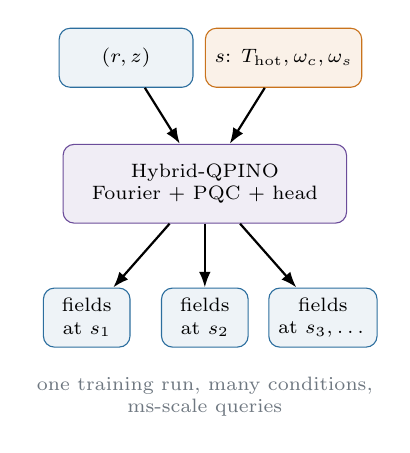
\begin{tikzpicture}[font=\scriptsize,
  b/.style={rounded corners,draw=cblue,fill=cblue!8,minimum width=1.7cm,minimum height=0.75cm,align=center},
  q/.style={rounded corners,draw=qpurple,fill=qpurple!10,minimum width=3.6cm,minimum height=1.0cm,align=center},
  arr/.style={-{Latex[length=2mm]},thick}]
\node[b] (x) at (-1.0,0) {$(r,z)$};
\node[b,draw=warnorange,fill=warnorange!10] (s) at (1.0,0) {$s$: $T_{\mathrm{hot}},\omega_c,\omega_s$};
\node[q] (m) at (0,-1.6) {Hybrid-QPINO\\Fourier + PQC + head};
\node[b,minimum width=1.1cm] (o1) at (-1.5,-3.3) {fields\\at $s_1$};
\node[b,minimum width=1.1cm] (o2) at (0,-3.3) {fields\\at $s_2$};
\node[b,minimum width=1.1cm] (o3) at (1.5,-3.3) {fields\\at $s_3,\dots$};
\draw[arr] (x)--(m); \draw[arr] (s)--(m);
\draw[arr] (m)--(o1); \draw[arr] (m)--(o2); \draw[arr] (m)--(o3);
\node[text=phgray,align=center] at (0,-4.3) {one training run, many conditions,\\ms-scale queries};
\end{tikzpicture}
\end{columns}
\end{frame}

% =====================================================================
\section{Benchmarks and protocol}
% =====================================================================

\begin{frame}{Benchmark 1: silicon CZ melt \pending}
\begin{columns}[T,onlytextwidth]
\column{0.34\textwidth}
\begin{center}
\footnotesize
\begin{tabular}{ll}
\toprule
Property & Value \\
\midrule
Reference & Axisymmetric CFD \\
Domain & $r\in[0,0.30]$\,m \\
 & $z\in[0,0.15]$\,m \\
Nodes & 18,108 \\
Outputs & $u_r,u_z,u_\theta,p,T$ \\
$T$ range & 1685--1750\,K \\
Split & 17,203 / 905 \\
\bottomrule
\end{tabular}
\end{center}
\begin{block}{Scope}
\scriptsize Steady, laminar, single-phase reference; geometry and BCs follow Huang et al.\ (2025).
\end{block}
\column{0.63\textwidth}
\centering
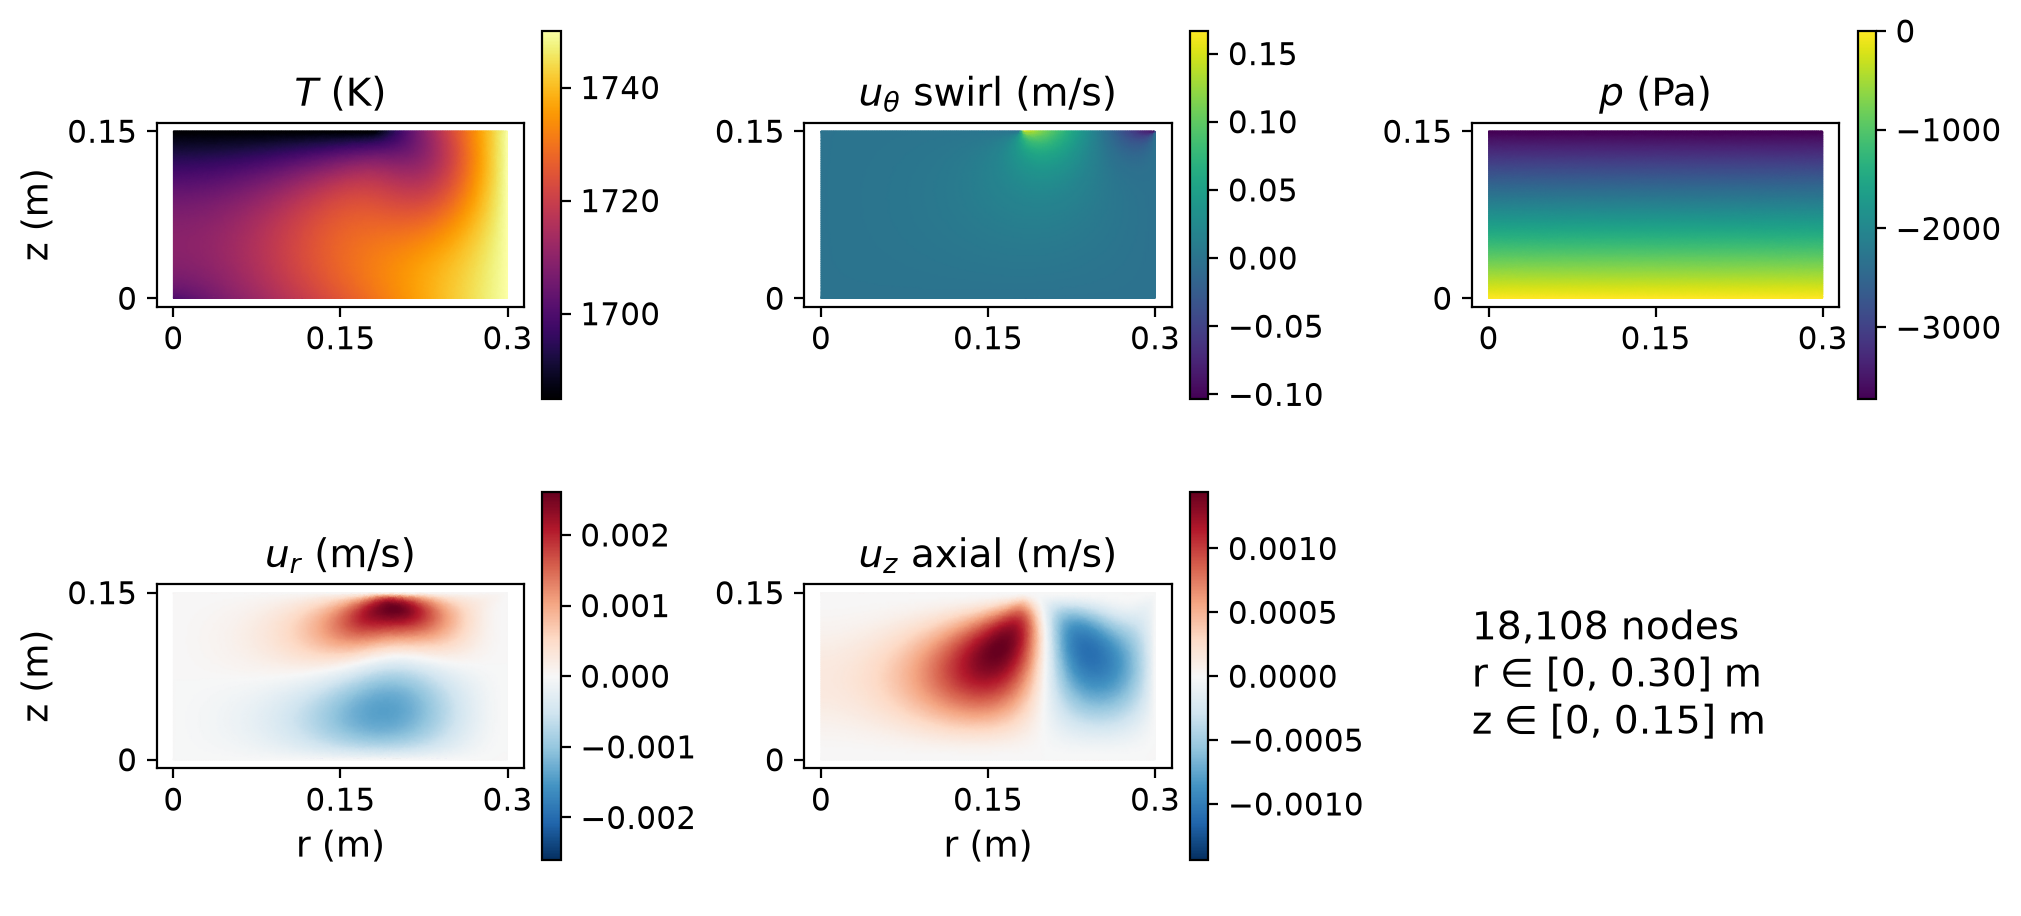
\includegraphics[width=\linewidth]{data_fields.png}
\figcap{Training data: $T$, swirl $u_\theta$, $p$, radial $u_r$ and axial $u_z$. Note the counter-rotating meridional cells and the thin swirl layer under the crystal.}
\begin{block}{Next physics}
\footnotesize Oxygen concentration transport (species equation) and the evolving melt--crystal interface.
\end{block}
\end{columns}
\end{frame}

\begin{frame}{Benchmark 2: LH$_2$ cryogenic boil-off \planned}
\begin{columns}[T,onlytextwidth]
\column{0.55\textwidth}
\begin{block}{Physics to capture}
\begin{itemize}\small
  \item Wall heat leak $\to$ natural-convection boundary layer and thermal stratification.
  \item Turbulent convection (RANS closure in the reference CFD).
  \item Liquid--vapour interface with evaporation (VOF + phase-change mass transfer).
  \item Outputs: velocity, temperature, phase fraction, boil-off rate, ullage pressure.
\end{itemize}
\end{block}
\begin{alertblock}{Status}
\small Benchmark and outputs defined; reference CFD data not yet generated.
\end{alertblock}
\column{0.41\textwidth}
\centering
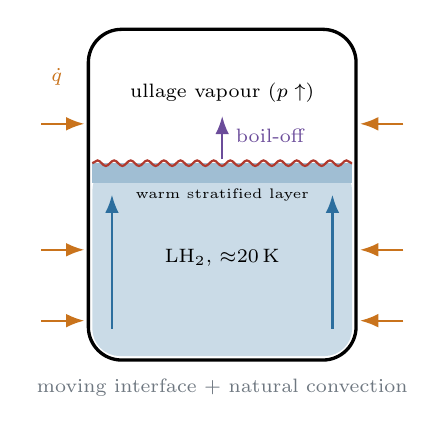
\begin{tikzpicture}[font=\scriptsize]
\draw[very thick,rounded corners=12pt] (0,0) rectangle (3.4,4.2);
\fill[cblue!25,rounded corners=10pt] (0.05,0.05) rectangle (3.35,2.5);
\fill[cblue!45] (0.05,2.25) rectangle (3.35,2.5);
\draw[qred,thick,decorate,decoration={snake,amplitude=1pt,segment length=6pt}] (0.05,2.5)--(3.35,2.5);
\node at (1.7,3.4) {ullage vapour ($p\uparrow$)};
\node at (1.7,1.3) {LH$_2$, $\approx$20\,K};
\node[font=\tiny] at (1.7,2.1) {warm stratified layer};
\foreach \y in {0.5,1.4,3.0}{\draw[-{Latex},warnorange,thick] (-0.6,\y)--(-0.05,\y);\draw[-{Latex},warnorange,thick] (4.0,\y)--(3.45,\y);}
\node[warnorange] at (-0.4,3.6) {$\dot q$};
\draw[-{Latex},thick,qpurple] (1.7,2.55)--(1.7,3.1);
\node[qpurple,anchor=west] at (1.75,2.85) {boil-off};
\draw[-{Latex},cblue,thick] (0.3,0.4)--(0.3,2.1);
\draw[-{Latex},cblue,thick] (3.1,0.4)--(3.1,2.1);
\node[text=phgray] at (1.7,-0.35) {moving interface + natural convection};
\end{tikzpicture}
\end{columns}
\end{frame}

\begin{frame}{Evaluation protocol and compute pipeline}
\begin{columns}[T,onlytextwidth]
\column{0.50\textwidth}
\begin{itemize}\footnotesize\setlength{\itemsep}{1pt}
  \item \textbf{Ablations:} classical-only at matched budget; random-feature layer in place of the PQC.
  \item \textbf{Baselines:} classical PINN and PINO, matched optimiser, sampling, seeds.
  \item \textbf{Generalisation:} hold out a whole operating condition.
  \item \textbf{Reporting:} per-field error, unweighted loss components.
  \item \textbf{Cost:} wall time to target error, inference latency.
\end{itemize}
\begin{center}
\footnotesize
\begin{tabular}{lll}
\toprule
Sweep & Range & Held out \\
\midrule
$T_{\mathrm{hot}}$ & 1730--1785\,K & 1780\,K \\
$\omega_c$ (crucible) & $-10$ to $-1$ rpm & $-4$ rpm \\
$\omega_s$ (crystal) & 4--20 rpm & 7 rpm \\
\bottomrule
\end{tabular}
\end{center}
\column{0.47\textwidth}
\centering
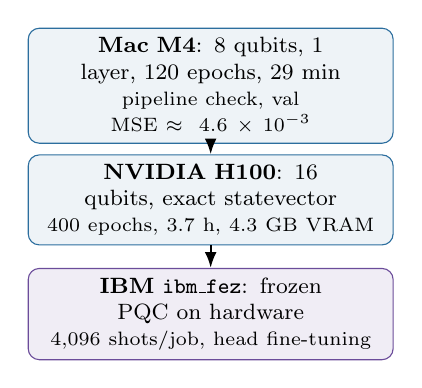
\begin{tikzpicture}[font=\footnotesize,
  st/.style={rounded corners,draw=cblue,fill=cblue!8,minimum width=4.6cm,minimum height=1.05cm,align=center,text width=4.4cm},
  sq/.style={rounded corners,draw=qpurple,fill=qpurple!10,minimum width=4.6cm,minimum height=1.05cm,align=center,text width=4.4cm},
  arr/.style={-{Latex[length=2mm]},thick}]
\node[st] (a) at (0,0) {\textbf{Mac M4}: 8 qubits, 1 layer, 120 epochs, 29 min \\\scriptsize pipeline check, val MSE $\approx4.6\times10^{-3}$};
\node[st] (b) at (0,-1.45) {\textbf{NVIDIA H100}: 16 qubits, exact statevector\\\scriptsize 400 epochs, 3.7 h, 4.3 GB VRAM};
\node[sq] (c) at (0,-2.9) {\textbf{IBM \texttt{ibm\_fez}}: frozen PQC on hardware\\\scriptsize 4,096 shots/job, head fine-tuning};
\draw[arr] (a)--(b); \draw[arr] (b)--(c);
\end{tikzpicture}
\vspace{0.1cm}
\begin{block}{Note}
\scriptsize 16 qubits = $2^{16}$ amplitudes: exactly simulable on one GPU. Hardware runs test noise robustness and deployment, not quantum advantage.
\end{block}
\end{columns}
\end{frame}

% =====================================================================
\section{Results}
% =====================================================================

\begin{frame}{Result 1: fast convergence in the data-driven phase \shown}
\begin{columns}[T,onlytextwidth]
\column{0.44\textwidth}
\begin{center}
\footnotesize
\begin{tabular}{llll}
\toprule
Epoch & Train loss & Val MSE & Val $T$ \\
\midrule
1  & $1.16\!\times\!10^{-2}$ & $4.83\!\times\!10^{-3}$ & $1.37\!\times\!10^{-3}$ \\
10 & $5.92\!\times\!10^{-5}$ & $3.11\!\times\!10^{-4}$ & $1.47\!\times\!10^{-4}$ \\
\textbf{20} & $\mathbf{5.26\!\times\!10^{-5}}$ & $\mathbf{1.58\!\times\!10^{-4}}$ & $\mathbf{5.07\!\times\!10^{-5}}$ \\
30 & $2.96\!\times\!10^{-5}$ & $1.75\!\times\!10^{-4}$ & $6.15\!\times\!10^{-5}$ \\
50 & $2.07\!\times\!10^{-5}$ & $2.13\!\times\!10^{-4}$ & $2.91\!\times\!10^{-5}$ \\
\bottomrule
\end{tabular}
\end{center}
\begin{block}{Reading}
\small Validation MSE drops \textbf{30$\times$ in 20 epochs}. Best checkpoint $1.58\times10^{-4}$ (random spatial split, in distribution).
\end{block}
\column{0.53\textwidth}
\centering
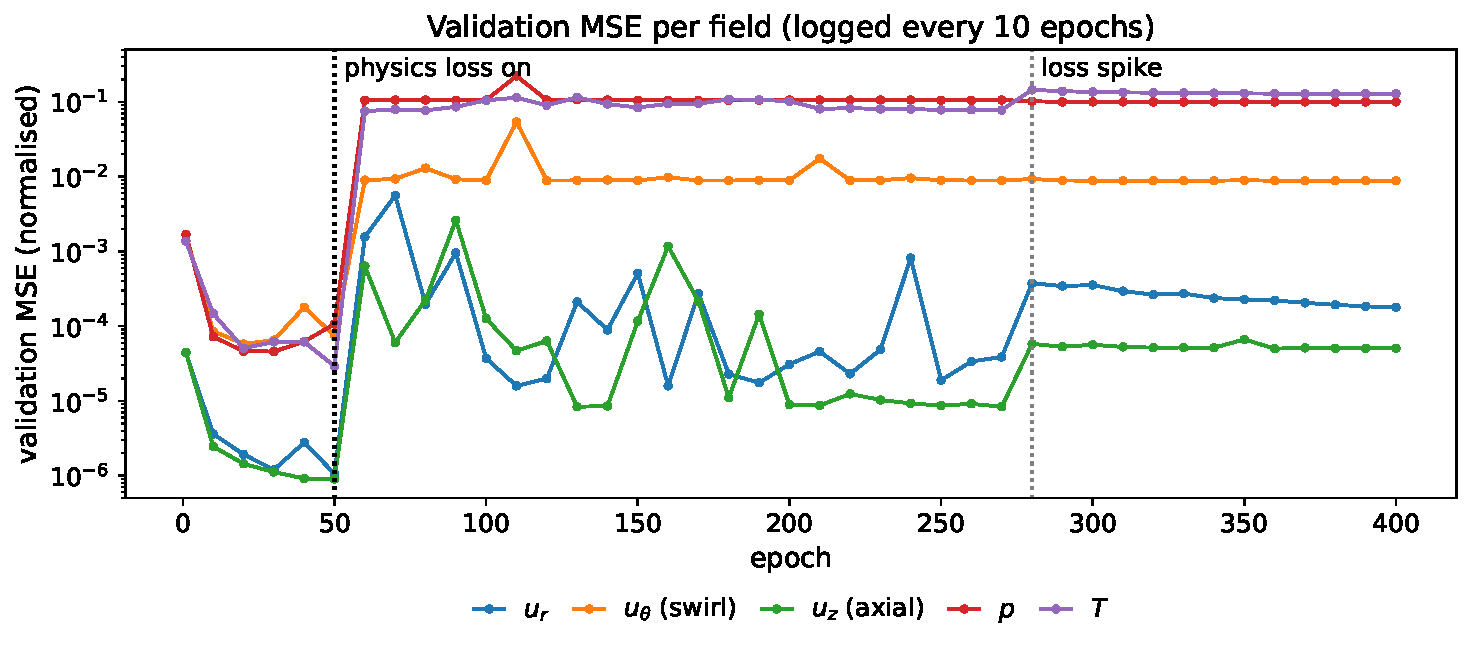
\includegraphics[width=\linewidth,height=0.72\textheight,keepaspectratio]{training_val_fields.pdf}
\figcap{Per-field validation MSE (H100, 400 epochs). Fields reach $10^{-6}$--$10^{-4}$ before the physics loss switches on at epoch 50.}
\end{columns}
\end{frame}

\begin{frame}{Result 2: thermal and swirl fields captured \shown}
\centering
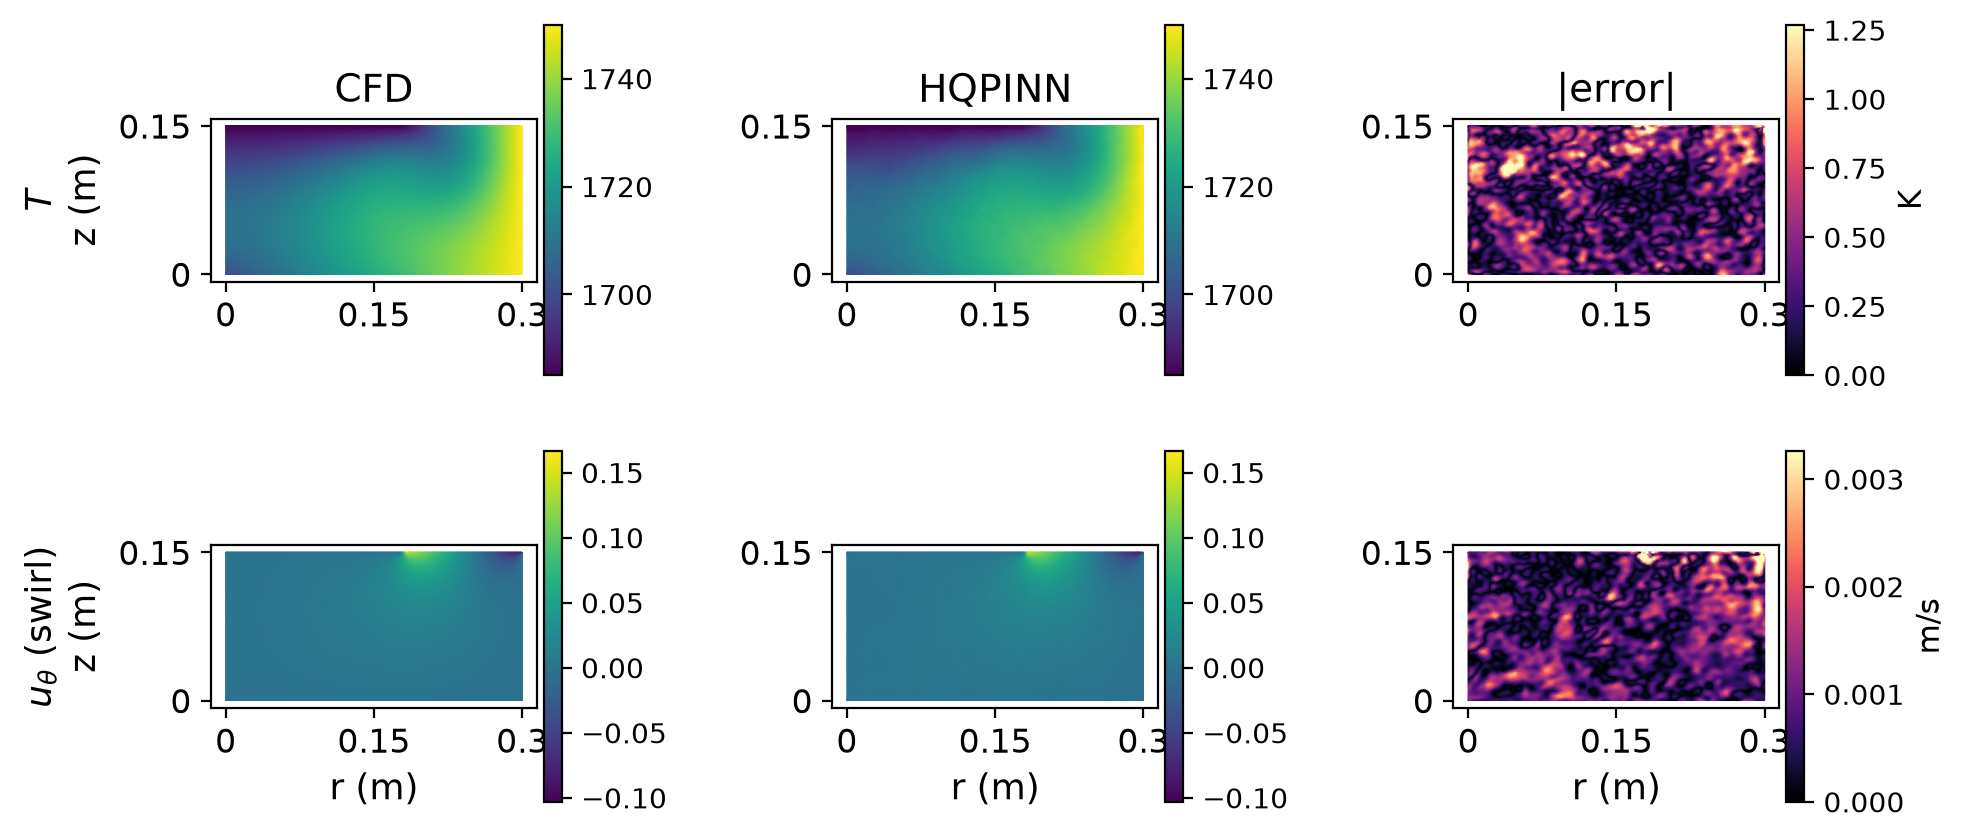
\includegraphics[width=0.86\linewidth,height=0.68\textheight,keepaspectratio]{field_maps_best_Tsw.png}
\figcap{CFD reference vs Hybrid-QPINN (best checkpoint) and absolute error: temperature $T$ (top, error $\lesssim$1.25\,K on a 65\,K range) and swirl $u_\theta$ (bottom, error $\lesssim3\times10^{-3}$\,m/s on $\pm0.15$\,m/s).}
\takeaway{The thin swirl layer under the rotating crystal and the hot-wall thermal gradient are both reproduced.}
\end{frame}

\begin{frame}{Result 2 (cont.): meridional velocities, the hardest fields \shown}
\begin{columns}[T,onlytextwidth]
\column{0.63\textwidth}
\centering
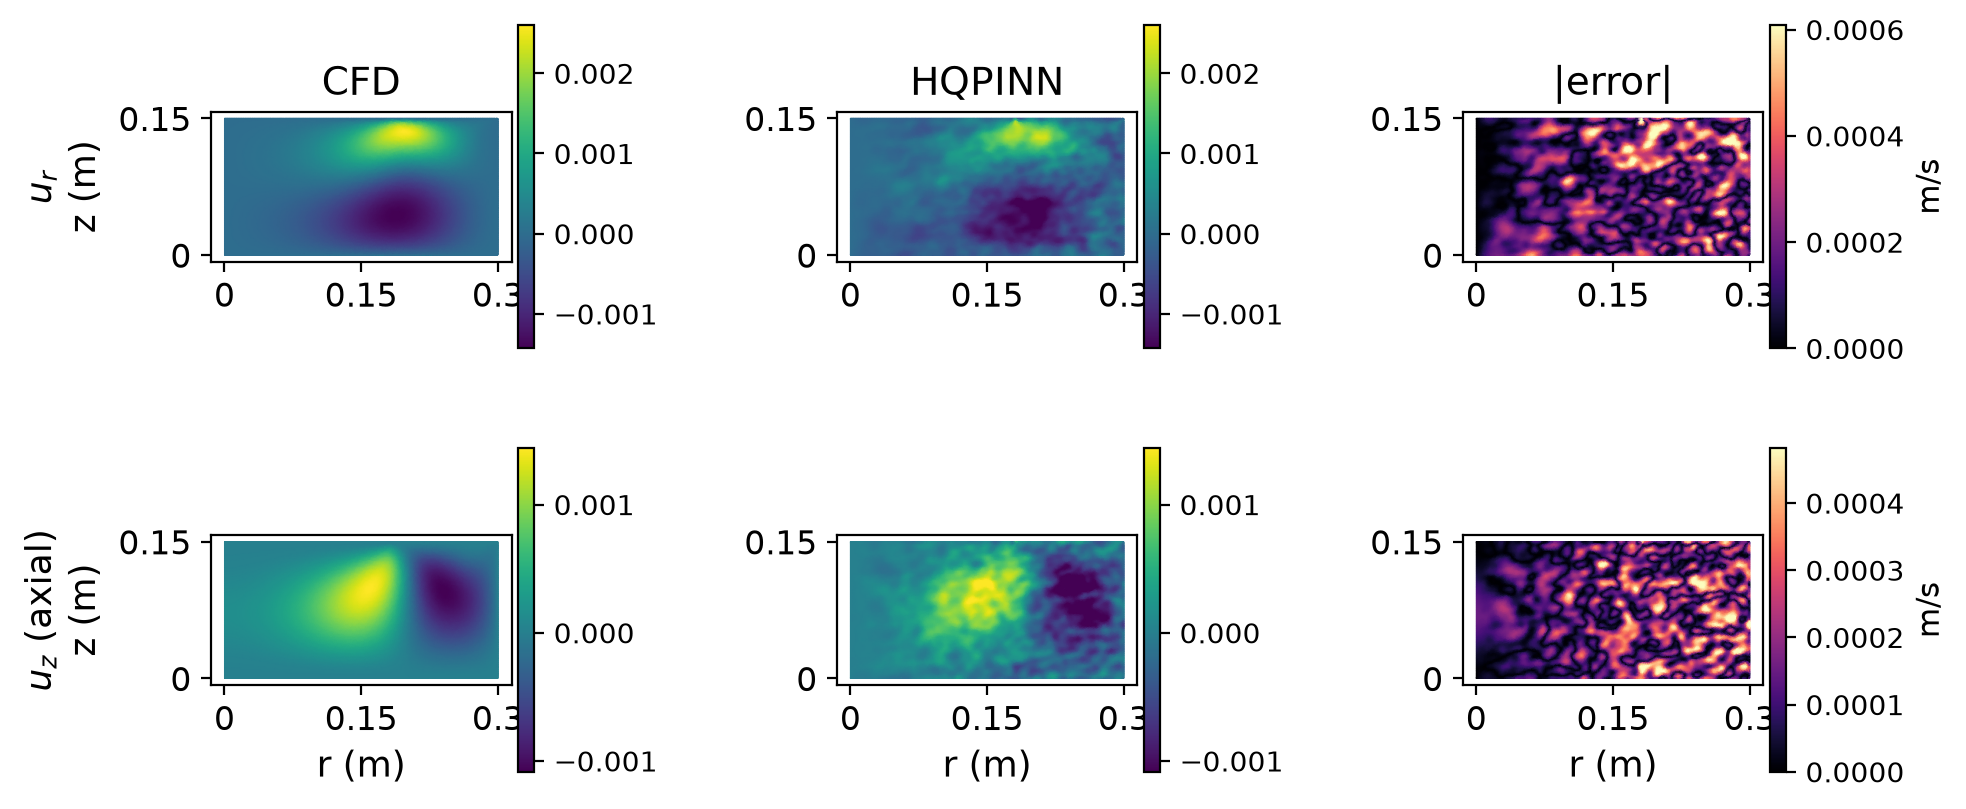
\includegraphics[width=\linewidth]{field_maps_best_urz.png}
\figcap{$u_r$ (top) and $u_z$ (bottom): CFD, Hybrid-QPINN, $|$error$|$.}
\column{0.34\textwidth}
\begin{center}
\footnotesize
\begin{tabular}{ll}
\toprule
Field & Val MSE (norm.) \\
\midrule
$u_r$ & $1.93\times10^{-6}$ \\
$u_z$ & $5.78\times10^{-5}$ \\
$u_\theta$ & $1.44\times10^{-6}$ \\
$p$ & $4.62\times10^{-5}$ \\
$T$ & $5.07\times10^{-5}$ \\
\bottomrule
\end{tabular}
\end{center}
\begin{itemize}\scriptsize
  \item Counter-rotating cells located correctly.
  \item Errors are small-scale and noisy: residual high-frequency content still to be learned.
\end{itemize}
\end{columns}
\end{frame}

\begin{frame}{Result 3: naive physics weighting destabilises training \shown}
\begin{columns}[T,onlytextwidth]
\column{0.52\textwidth}
\begin{center}
\footnotesize
\begin{tabular}{lllr}
\toprule
Field & Best (ep.\,20) & Final (ep.\,400) & Factor \\
\midrule
$u_r$ & $1.93\times10^{-6}$ & $1.79\times10^{-4}$ & 93$\times$ \\
$u_z$ & $5.78\times10^{-5}$ & $8.83\times10^{-3}$ & 153$\times$ \\
$u_\theta$ & $1.44\times10^{-6}$ & $5.06\times10^{-5}$ & 35$\times$ \\
$p$ & $4.62\times10^{-5}$ & $0.100$ & \textbf{2,165$\times$} \\
$T$ & $5.07\times10^{-5}$ & $0.129$ & \textbf{2,544$\times$} \\
\bottomrule
\end{tabular}
\end{center}
{\scriptsize\ttfamily
{[0280]} loss=1.04e+09 data=5.06e-02 phys=2.16e+10\\
{[0290]} loss=1.18e+14 data=4.97e-02 phys=2.15e+15\\
{[0300]} loss=5.57e-02 data=4.85e-02 phys=9.62e-02}
\column{0.44\textwidth}
\begin{alertblock}{Diagnosis}
\small Data loss stays near 0.05; the blow-up is entirely in the physics residual (jump at epoch 50, spike at 280 in Result 1's plot). Root cause: the $p_{\mathrm{coeff}}$ scale mismatch.
\end{alertblock}
\begin{exampleblock}{Fixes under test \pending}
\small Physics weight 0.001--0.005; per-field pressure residual scaling; re-check pressure nondimensionalisation.
\end{exampleblock}
\end{columns}
\end{frame}

\begin{frame}{Result 4: the circuit runs on real quantum hardware \shown}
\begin{columns}[T,onlytextwidth]
\column{0.60\textwidth}
\centering
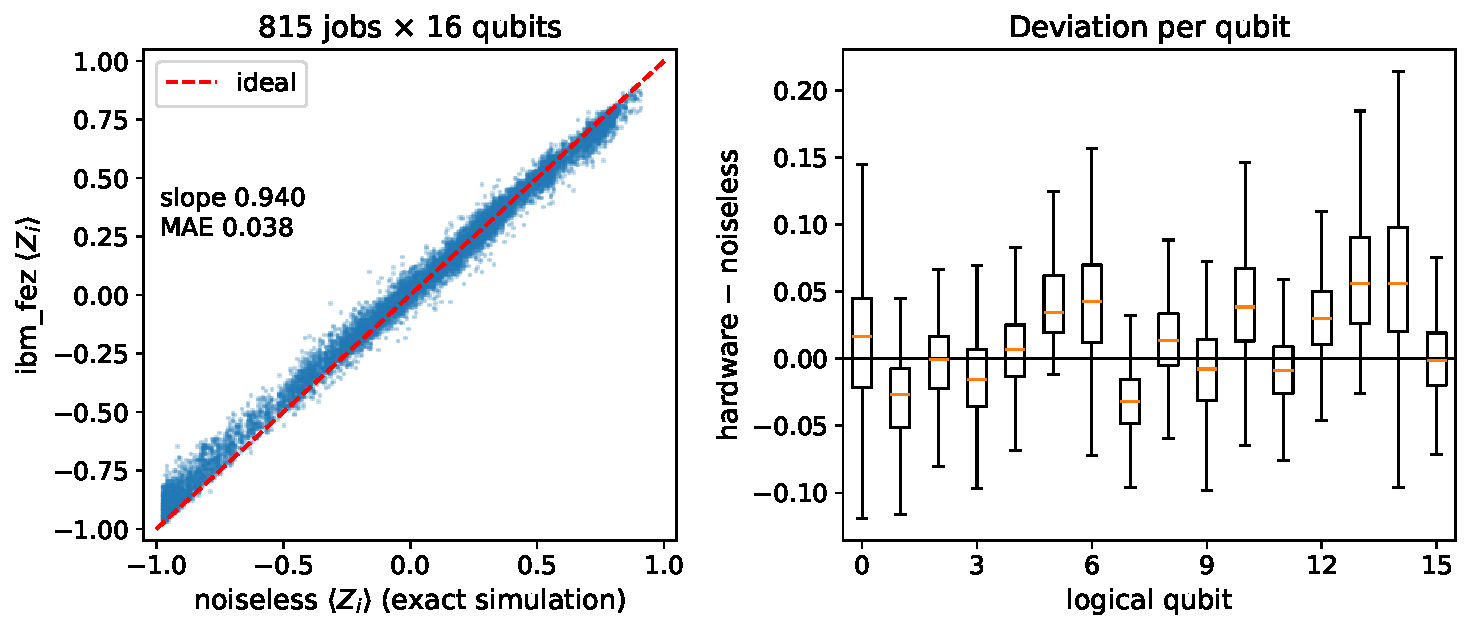
\includegraphics[width=\linewidth,height=0.62\textheight,keepaspectratio]{ibm_hw_vs_sim.pdf}
\figcap{\texttt{ibm\_fez} vs exact simulation, 815 jobs $\times$ 16 qubits: slope 0.940, MAE 0.038; per-qubit deviation stays within about $\pm$0.1.}
\column{0.37\textwidth}
\begin{center}
\scriptsize
\begin{tabular}{ll}
\toprule
Fine-tuning session & Value \\
\midrule
Backend & \texttt{ibm\_fez} (156 q) \\
Jobs completed / failed & \textbf{500 / 0} \\
Shots per job & 4,096 \\
Total shots & 2,048,000 \\
Session & 125 min \\
Trainable scope & head (19,205) \\
\bottomrule
\end{tabular}
\end{center}
\begin{block}{Reading}
\scriptsize Hardware features are a mildly compressed (slope $<1$), low-bias copy of the simulated ones. Strategy: freeze the PQC, re-adapt the classical head on hardware $\langle Z_i\rangle$. \pending
\end{block}
\end{columns}
\end{frame}

\begin{frame}{Inside the trained circuit}
\begin{columns}[T,onlytextwidth]
\column{0.58\textwidth}
\centering
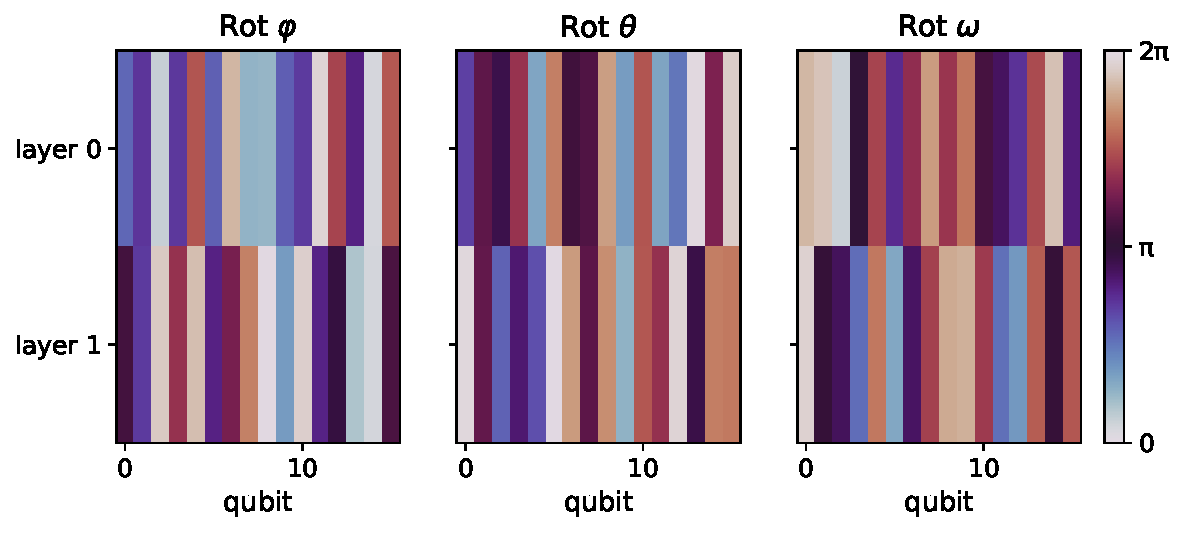
\includegraphics[width=\linewidth,height=0.6\textheight,keepaspectratio]{quantum_weights_heatmap.pdf}
\figcap{Trained Rot angles $(\varphi,\vartheta,\omega)$ per qubit, layers 0 and 1.}
\column{0.39\textwidth}
\begin{itemize}\small\setlength{\itemsep}{3pt}
  \item Angles span the full $[0,2\pi]$ range (mean 3.49, std 1.79 rad).
  \item No qubit stuck at a degenerate value; the two layers learn different patterns.
  \item In a longer run, LayerNorm weights qubits unequally ($\gamma\approx0.3$--$1.2$): the head relies on some quantum features more than others.
\end{itemize}
\end{columns}
\takeaway{The circuit is active and differentiated. Whether it adds accuracy is what the ablation will decide.}
\end{frame}

\begin{frame}{Parametric exploration: what a classical surrogate gives today}
\begin{columns}[T,onlytextwidth]
\column{0.44\textwidth}
\begin{block}{GPR baseline, held-out case}
\scriptsize Learns $(r,z,s)\mapsto$ fields; NRMSE = RMSE / std of the field.
\end{block}
\centering
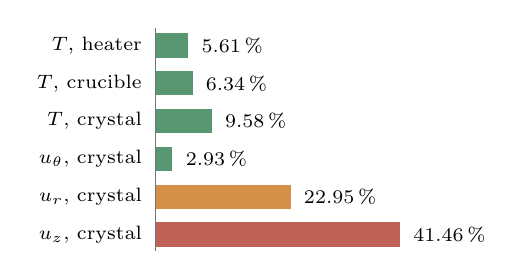
\begin{tikzpicture}[x=0.075cm,y=0.48cm,font=\scriptsize]
\foreach \lab/\val/\col [count=\i] in {%
  {$T$, heater}/5.61/okgreen,
  {$T$, crucible}/6.34/okgreen,
  {$T$, crystal}/9.58/okgreen,
  {$u_\theta$, crystal}/2.93/okgreen,
  {$u_r$, crystal}/22.95/warnorange,
  {$u_z$, crystal}/41.46/qred}{%
  \fill[\col!80] (0,-\i-0.32) rectangle (\val,-\i+0.32);
  \node[anchor=east] at (-0.6,-\i) {\lab};
  \node[anchor=west] at (\val+0.6,-\i) {\val\,\%};
}
\draw[phgray] (0,-0.55)--(0,-6.45);
\end{tikzpicture}
\column{0.53\textwidth}
\centering
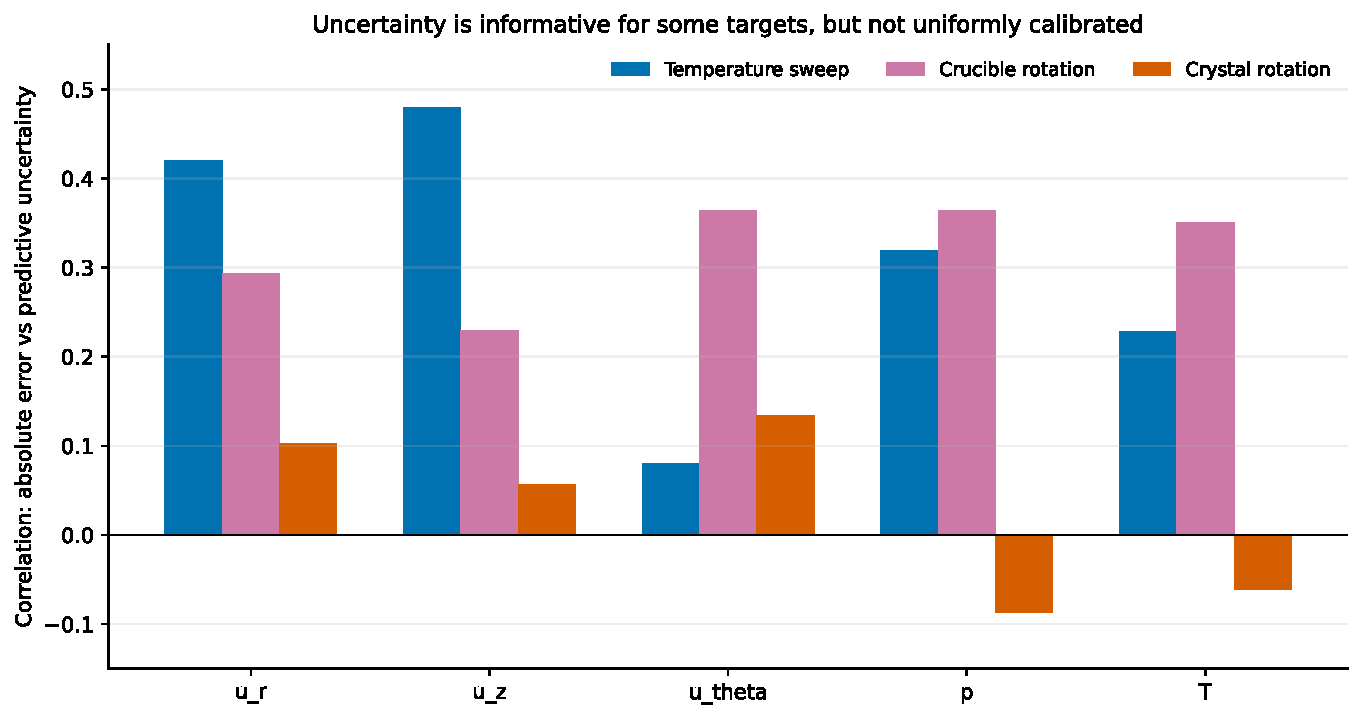
\includegraphics[width=\linewidth,height=0.55\textheight,keepaspectratio]{gpr_uncertainty.pdf}
\figcap{Correlation between GPR predictive uncertainty and actual error, per field and sweep.}
\end{columns}
\takeaway{$T$ generalises (5.6--9.6\%); meridional velocities under crystal rotation do not (23--41\%). This is the bar QPINO must beat.}
\end{frame}

% =====================================================================
\section{Outlook}
% =====================================================================

\begin{frame}{Where the evidence stands today}
\renewcommand{\arraystretch}{1.08}
\footnotesize
\begin{tabular}{p{0.42\textwidth} p{0.13\textwidth} p{0.38\textwidth}}
\toprule
Claim & Status & Evidence \\
\midrule
Hybrid pipeline runs on GPU and real QPU & \shown & 500/500 IBM jobs; HW vs sim MAE 0.038 \\
Five coupled CZ fields fitted in distribution & \shown & Val MSE $1.58\times10^{-4}$ \\
Fast early convergence & \shown & 30$\times$ drop in 20 epochs \\
Physics loss needs field-aware scaling & \shown & 2,000$\times$ degradation for $p,T$ \\
Faster convergence than classical PINN/PINO & \pending & Matched baseline running \\
PQC adds accuracy over classical features & \pending & Ablation + random-feature control \\
Sharper generalisation across conditions & \planned & Case-wise holdout vs GPR / PINO \\
Reduced computational cost & \planned & GPU-hours to target error \\
Concentration, evolving interfaces, LH$_2$ & \planned & Species eq., interface tracking \\
\bottomrule
\end{tabular}
\takeaway{Early indications are positive; the hybrid-vs-classical advantage is decided by the matched ablations.}
\end{frame}

\begin{frame}{Next experiments}
\renewcommand{\arraystretch}{1.1}
\small
\centering
\begin{tabular}{llr}
\toprule
Priority & Experiment & Compute \\
\midrule
Critical & Classical-only baseline, matched parameters & 1$\times$H100, $\sim$4 h \\
Critical & Random-feature control in place of the PQC & 1$\times$H100, $\sim$4 h \\
Critical & Retrain with physics weight 0.001--0.005 & 1$\times$H100, $\sim$4 h \\
High & Physics gradients through the PQC (parameter shift) & architecture change \\
High & Case-wise holdout on three CZ sweeps (QPINO) & 3 runs \\
High & Complete head fine-tuning on IBM hardware & $\sim$500 jobs \\
Medium & LH$_2$ boil-off reference CFD + surrogate & CFD + H100 \\
\bottomrule
\end{tabular}
\end{frame}

\begin{frame}{Pathway to real-time digital twins}
\centering
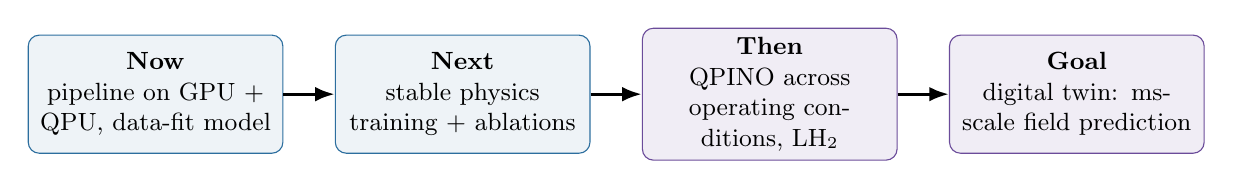
\begin{tikzpicture}[
  font=\small,
  st/.style={rounded corners,draw=cblue,fill=cblue!8,minimum width=3.2cm,minimum height=1.5cm,align=center,text width=3.0cm},
  sq/.style={rounded corners,draw=qpurple,fill=qpurple!10,minimum width=3.2cm,minimum height=1.5cm,align=center,text width=3.0cm},
  arr/.style={-{Latex[length=2.5mm]},very thick}
]
\node[st] (a) at (0,0) {\textbf{Now}\\pipeline on GPU + QPU, data-fit model};
\node[st] (b) at (3.9,0) {\textbf{Next}\\stable physics training + ablations};
\node[sq] (c) at (7.8,0) {\textbf{Then}\\QPINO across operating conditions, LH$_2$};
\node[sq] (d) at (11.7,0) {\textbf{Goal}\\digital twin: ms-scale field prediction};
\draw[arr] (a)--(b); \draw[arr] (b)--(c); \draw[arr] (c)--(d);
\end{tikzpicture}

\vspace{0.4cm}
\begin{columns}[T,onlytextwidth]
\column{0.32\textwidth}
\begin{block}{Data engine}
\footnotesize Agentic CFD (AutoFOAM) generates verified training cases from one prompt.
\end{block}
\column{0.32\textwidth}
\begin{block}{Surrogate}
\footnotesize Hybrid-QPINO trained once, queried across the full process window for parametric exploration.
\end{block}
\column{0.32\textwidth}
\begin{block}{Validator}
\footnotesize Physics residuals, uncertainty and benchmark checks before any prediction is trusted.
\end{block}
\end{columns}
\end{frame}

\begin{frame}{Key takeaways}
\begin{enumerate}\setlength{\itemsep}{5pt}
  \item \textbf{Framework:} Fourier features + data re-uploading + a shallow 16-qubit PQC (96 angles) as a trainable feature map inside a physics-informed network.
  \item \textbf{Demonstrated:} all five coupled CZ fields fitted (val MSE $1.58\times10^{-4}$, 30$\times$ drop in 20 epochs); the circuit runs on IBM hardware (500/500 jobs, MAE 0.038 vs simulation).
  \item \textbf{Learned:} physics weighting must respect field scales; a pressure coefficient of $\sim\!10^5$ can wreck training.
  \item \textbf{Being tested:} faster convergence, sharper generalisation and lower cost than classical PINN/PINO, via matched ablations.
  \item \textbf{Destination:} QPINO surrogates for crystal growth and LH$_2$ storage as the core of real-time digital twins.
\end{enumerate}
\end{frame}

\begin{frame}{References}
\scriptsize
\begin{itemize}\setlength{\itemsep}{1pt}
  \item Raissi, Perdikaris, Karniadakis, \emph{Physics-informed neural networks}, J.\ Comput.\ Phys.\ (2019).
  \item Rahaman et al., \emph{On the spectral bias of neural networks}, ICML 2019.
  \item Tancik et al., \emph{Fourier features let networks learn high frequency functions}, NeurIPS 2020.
  \item P\'erez-Salinas et al., \emph{Data re-uploading for a universal quantum classifier}, Quantum (2020).
  \item Schuld, Sweke, Meyer, \emph{Effect of data encoding on the expressive power of variational quantum machine-learning models}, PRA (2021).
  \item Wang, Teng, Perdikaris, \emph{Understanding and mitigating gradient pathologies in PINNs}, SIAM J.\ Sci.\ Comput.\ (2021).
  \item Krishnapriyan et al., \emph{Characterizing possible failure modes in PINNs}, NeurIPS 2021.
  \item Li et al., \emph{Physics-informed neural operator for learning PDEs} (2021).
  \item Huang, Cao, Liu, Liu, \emph{Thermal-fluid coupling in Czochralski silicon growth based on an improved PINN}, AIP Advances 15, 105202 (2025).
  \item Chapagain et al., \emph{Component-level evaluation of adaptive PINN training for CFD-oriented crystal growth simulation}, NeurIPS 2026 Sim2Science workshop.
  \item Neelan, Seshaditya, \emph{AutoFOAM: the self-refining autonomous OpenFOAM agent}.
\end{itemize}
\end{frame}

\begin{frame}
\centering
\Large\textbf{Thank you}

\vspace{0.3cm}
\normalsize Questions?

\vspace{0.6cm}
\footnotesize
\textbf{Acknowledgements:} Niruta Chapagain, Rohit Raj (adaptive PINN study);
Bertwin Kurisinkal Shine, TU Chemnitz (CZ reference CFD);
Arun Govind Neelan (AutoFOAM); A Seshaditya, QuaSi Berlin (physics-informed ML).
\end{frame}

\end{document}
